%% 使用 njuthesis 文档类生成南京大学学位论文的示例文档
%%
%% 作者:胡海星,starfish (at) gmail (dot) com
%% 项目主页: http://haixing-hu.github.io/nju-thesis/
%%
%% 本样例文档中用到了吕琦同学的博士论文的提高和部分内容,在此对他表示感谢。
%%
\documentclass[master,winfonts]{njuthesis}
%% njuthesis 文档类的可选参数有:
%%   nobackinfo 取消封二页导师签名信息。注意,按照南大的规定,是需要签名页的。
%%   phd/master/bachelor 选择博士/硕士/学士论文

% 使用 blindtext 宏包自动生成章节文字
% 这仅仅是用于生成样例文档,正式论文中一般用不到该宏包
%\input{preamble}


% 使用 blindtext 宏包自动生成章节文字
% 这仅仅是用于生成样例文档,正式论文中一般用不到该宏包
\usepackage{url}
\usepackage{verbatim}
\usepackage[math]{blindtext}
\usepackage{listings}
\usepackage{color}
\usepackage[figuresright]{rotating}
\renewcommand{\multirowsetup}{\centering} 
\usepackage{multirow}

\usepackage{tablefootnote}
\usepackage{graphicx}
\usepackage{tikzscale}
\usepackage{threeparttable}
\usepackage{ulem}
\newcommand{\li}{\uline{\hspace{0.5em}}}
\usepackage[ruled,lined,linesnumbered,vlined,algo2e,boxed]{algorithm2e}
\renewcommand{\listalgorithmcfname}{算法列表}
\renewcommand{\algorithmcfname}{算法}
\renewcommand*{\thealgocf}{{\thechapter}-%\kern.07em\rule[.5ex]{.4em}{.15ex}\kern.07em
{\arabic{algocf}}}
\SetKwInput{KwIn}{输入}
\SetKwInput{KwOut}{输出}

\definecolor{dkgreen}{rgb}{0,0.6,0}
\definecolor{gray}{rgb}{0.5,0.5,0.5}
\definecolor{mauve}{rgb}{0.58,0,0.82}
\lstset{frame=tb,
  language=Java,
  basicstyle=\footnotesize\ttfamily,
  aboveskip=3mm,
  belowskip=3mm,
  %xleftmargin=2em,
  xleftmargin=12em,
  xrightmargin=10em,
  showstringspaces=false,
  columns=flexible,
  %basicstyle={\small\ttfamily},
  numbers=left,
  numberstyle=\footnotesize,
  %numberstyle=\tiny\color{gray},
  %numberstyle={\color[RGB]{0,192,192}\small},
  keywordstyle=\color{blue},
  commentstyle=\color{dkgreen},
  stringstyle=\color{mauve},
  breaklines=true,
  breakatwhitespace=true
  tabsize=3
}

%\usepackage{bera}% optional: just to have a nice mono-spaced font
\usepackage{xcolor}
\colorlet{punct}{red!60!black}
\definecolor{background}{HTML}{EEEEEE}
\definecolor{delim}{RGB}{20,105,176}
\colorlet{numb}{magenta!60!black}

\lstdefinelanguage{json}{
    basicstyle=\normalfont\ttfamily,
    numbers=left,
    numberstyle=\scriptsize,
    stepnumber=1,
    numbersep=8pt,
    showstringspaces=false,
    breaklines=true,
    frame=lines,
    %backgroundcolor=\color{background},
    literate=
     *{0}{{{\color{numb}0}}}{1}
      {1}{{{\color{numb}1}}}{1}
      {2}{{{\color{numb}2}}}{1}
      {3}{{{\color{numb}3}}}{1}
      {4}{{{\color{numb}4}}}{1}
      {5}{{{\color{numb}5}}}{1}
      {6}{{{\color{numb}6}}}{1}
      {7}{{{\color{numb}7}}}{1}
      {8}{{{\color{numb}8}}}{1}
      {9}{{{\color{numb}9}}}{1}
      {:}{{{\color{punct}{:}}}}{1}
      {,}{{{\color{punct}{,}}}}{1}
      {\{}{{{\color{delim}{\{}}}}{1}
      {\}}{{{\color{delim}{\}}}}}{1}
      {[}{{{\color{delim}{[}}}}{1}
      {]}{{{\color{delim}{]}}}}{1},
}


\usepackage{tikz}
\usepackage{pgfplots}
\usepackage{threeparttable}
\usepackage{makecell}
\usepackage{footnote}
% Please add the following required packages to your document preamble:
\usepackage{booktabs}
\usepackage{pgfplots}
\usepgfplotslibrary{statistics}
%Define the color series
\definecolor{RYB1}{RGB}{230,97,1}
\definecolor{RYB2}{RGB}{65,105,225}
\definecolor{RYB3}{RGB}{200,150,250}
\pgfplotscreateplotcyclelist{colorbrewer-RYB}{
{RYB1!50!black,fill=RYB1},
{RYB2!50!black,fill=RYB2},
{RYB3!50!black,fill=RYB3}} 
%\pgfplotsset{compat=1.8}

\usepackage[math]{blindtext}
\usepackage{algorithm}
\usepackage{algorithmic}
\usepackage{url}
\usepackage{hyperref}



%%%%%%%%%%%%%%%%%%%%%%%%%%%%%%%%%%%%%%%%%%%%%%%%%%%%%%%%%%%%%%%%%%%%%%%%%%%%%%%
% 设置论文的中文封面

% 论文标题,不可换行
\title{基于ProgrammableWeb网站的Web服务推荐研究}
\titlea{基于ProgrammableWeb网站的}
\titleb{Web服务推荐研究}
%\titleb{web服务推荐算法研究}

% 如果论文标题过长,可以分两行,第一行用\titlea{}定义,第二行用\titleb{}定义,将上面的\title{}注释掉
% \titlea{半轻衰变$D^+\to \omega(\phi)e^+\nu_e$的研究}
% \titleb{和弱衰变$J/\psi \to D_s^{(*)-}e^+\nu_e$的寻找}

% 论文作者姓名
\author{王勇}
% 论文作者联系电话
\telphone{15651826383}
% 论文作者电子邮件地址
\email{1558448539@qq.com}
% 论文作者学生证号
\studentnum{MF1533054}
% 论文作者入学年份(年级)
\grade{2018}
\startyear{2015}
% 导师姓名职称
\supervisor{胡昊~~副教授}
% 导师的联系电话
\supervisortelphone{18913961638}
% 论文作者的学科与专业方向
\major{计算机技术}
% 论文作者的研究方向
\researchfield{服务计算}
% 论文作者所在院系的中文名称
\department{计算机科学与技术系}
% 论文作者所在学校或机构的名称。此属性可选,默认值为``南京大学''。
\institute{南京大学}
% 论文的提交日期,需设置年、月、日。
\submitdate{2018年8月21日}
% 论文的答辩日期,需设置年、月、日。
\defenddate{2018年8月23日}
% 论文的定稿日期,需设置年、月、日。此属性可选,默认值为最后一次编译时的日期,精确到日。
%% \date{2013年5月1日}

%%%%%%%%%%%%%%%%%%%%%%%%%%%%%%%%%%%%%%%%%%%%%%%%%%%%%%%%%%%%%%%%%%%%%%%%%%%%%%%
% 设置论文的英文封面

% 论文的英文标题,不可换行
\englishtitle{Research on Web Service Recommendation Based on ProgrammableWeb}
% 论文作者姓名的拼音
\englishauthor{Wang Yong}
% 导师姓名职称的英文
\englishsupervisor{Associate Professor Hu Hao}
% 论文作者学科与专业的英文名
\englishmajor{Computer Technology}
% 论文作者所在院系的英文名称

\englishdepartment{Department of Computer Science and Technology}
% 论文作者所在学校或机构的英文名称。此属性可选,默认值为``Nanjing University''。
\englishinstitute{Nanjing University}
% 论文完成日期的英文形式,它将出现在英文封面下方。需设置年、月、日。日期格式使用美国的日期
% 格式,即``Month day, year'',其中``Month''为月份的英文名全称,首字母大写;``day''为
% 该月中日期的阿拉伯数字表示;``year''为年份的四位阿拉伯数字表示。此属性可选,默认值为最后
% 一次编译时的日期。
\englishdate{August 23, 2018}

%%%%%%%%%%%%%%%%%%%%%%%%%%%%%%%%%%%%%%%%%%%%%%%%%%%%%%%%%%%%%%%%%%%%%%%%%%%%%%%
% 设置论文的中文摘要

% 设置中文摘要页面的论文标题及副标题的第一行。
% 此属性可选,其默认值为使用|\title|命令所设置的论文标题
 \abstracttitlea{基于ProgrammableWeb网站的Web服务推荐研究}
% 设置中文摘要页面的论文标题及副标题的第二行。
% 此属性可选,其默认值为空白
 \abstracttitleb{}

%%%%%%%%%%%%%%%%%%%%%%%%%%%%%%%%%%%%%%%%%%%%%%%%%%%%%%%%%%%%%%%%%%%%%%%%%%%%%%%
% 设置论文的英文摘要

% 设置英文摘要页面的论文标题及副标题的第一行。
% 此属性可选,其默认值为使用|\englishtitle|命令所设置的论文标题
\englishabstracttitlea{Research on Web Service Recommendation }
% 设置英文摘要页面的论文标题及副标题的第二行。
% 此属性可选,其默认值为空白
\englishabstracttitleb{Based on ProgrammableWeb}

%%%%%%%%%%%%%%%%%%%%%%%%%%%%%%%%%%%%%%%%%%%%%%%%%%%%%%%%%%%%%%%%%%%%%%%%%%%%%%%
\begin{document}

%%%%%%%%%%%%%%%%%%%%%%%%%%%%%%%%%%%%%%%%%%%%%%%%%%%%%%%%%%%%%%%%%%%%%%%%%%%%%%%
% 制作中文封面
\maketitle
% 制作英文封面
\makeenglishtitle


%%%%%%%%%%%%%%%%%%%%%%%%%%%%%%%%%%%%%%%%%%%%%%%%%%%%%%%%%%%%%%%%%%%%%%%%%%%%%%%
% 开始前言部分
\frontmatter

%%%%%%%%%%%%%%%%%%%%%%%%%%%%%%%%%%%%%%%%%%%%%%%%%%%%%%%%%%%%%%%%%%%%%%%%%%%%%%%
% 论文的中文摘要
\begin{abstract}
随着面向服务架构的快速发展,互联网上开始出现大量的Web服务,面对Web服务数量快速增长带来的信息爆炸的现状,服务推荐成为了服务计算领域一个热门的研究问题。伴随着Web服务数量的飞速增长,以ProgrammableWeb\footnote{https://www.programmableweb.com/}网站为代表的服务平台逐渐成为了Web服务发布和发现的主要中介,面对服务平台上大量的Web服务,用户往往由于经验或能力的不足而难以选择,为用户推荐合适的Web服务成为了当务之急。

当前Web服务推荐大都关注服务的功能信息或者服务质量QoS、时间等非功能信息,对于Web服务自身丰富的边缘信息,例如主题信息、服务组合信息等没有给予足够的重视。同时,目前的服务推荐算法往往只致力于准确性的提高,对于推荐算法的多样性则很少关注,这将导致服务平台产生较多的长尾服务。针对目前Web服务推荐方法存在的不足,本文基于服务平台ProgrammableWeb,在准确性和多样性方面作了如下工作:

\begin{enumerate}
\item 在准确性方面,提出了一种基于主题信息和服务组合信息的Web服务推荐算法,该算法基于ProgrammableWeb网站的真实数据,通过用户的隐式反馈来提取用户的兴趣偏好,通过将Web服务的功能主题信息和服务组合信息融合进矩阵分解模型,以更好地预测用户兴趣评分。实验表明,与现有的协同过滤算法相比,我们的算法在准确性上取得了一定的提升。

\item 在多样性方面,提出了一种考虑用户偏差的改进重排名算法以提高推荐的多样性,该算法考虑了用户评分习惯差异性和用户兴趣分布差异性,并将这两种偏差结合进了阈值$T_R$的计算中,使得改进的重排名模型不再按照固定阈值$T_R$,而是通过考虑了用户差异性的个性化阈值来为用户提高多样性。实验表明,与经典的重排名算法相比,该算法可以在牺牲少量准确性的基础上,大幅提高Web服务推荐的多样性。
\end{enumerate}

% 中文关键词。关键词之间用中文全角分号隔开,末尾无标点符号。
\keywords{服务推荐;边缘信息;主题;服务组合信息;矩阵分解;多样性}
\end{abstract}

%%%%%%%%%%%%%%%%%%%%%%%%%%%%%%%%%%%%%%%%%%%%%%%%%%%%%%%%%%%%%%%%%%%%%%%%%%%%%%%
% 论文的英文摘要
\begin{englishabstract}
With the development of SOA (Service Oriented Architecture), an increasing number of Web services
have been published on the Internet, which leads to information overload. How to recommend suitable Web services for users becomes a research hotspot in service computing. Currently ProgrammableWeb has become the main intermediary for service publishing and discovery. Thus in this paper we focus on how to recommend suitable Web services for users on ProgrammableWeb.

The current Web service recommendation methods mainly focus on QoS (Quality of Service) or the functional information of services. These methods pay little attention to rich side information of Web services, such as topic information and compositional information. Furthermore, current service recommendation methods tend to focus only on the improvement of accuracy, while neglecting the recommendation diversity. This situation will lead to more long tail services generated on the service platform. To address the discussed issues, this paper has done the following work based on ProgrammableWeb:

\begin{enumerate}
\item To improve the recommendation accuracy, we propose an algorithm based on topic information and compositional information of services. The algorithm is based on the real-world data from ProgrammableWeb. The implicit user feedback is used to calculate the ratings, and the topic information and compositional information of service is integrated to the matrix factorization model to predict users' ratings. The experimental results show that the proposed algorithm outperforms the existing collaborative filtering algorithms on the recommendation accuracy.
\item To improve the recommendation diversity, we propose a re-ranking algorithm that considers user bias. The algorithm considers the biases in user scoring habits and user interest distribution, and combines these two biases into the calculation of the threshold $T_R$. Thus, the improved re-ranking model no longer improve the diversity according to the fixed threshold $T_R$. Experiments show that compared with the classical re-ranking algorithm, our methods can improve the diversity of Web service recommendation while maintaining acceptable levels of recommendation accuracy.

\end{enumerate}
% 英文关键词。关键词之间用英文半角逗号隔开,末尾无符号。
\englishkeywords{Service Recommendation, Side Information, Topic, Compositional Information, Matrix Factorization, Diversity}
\end{englishabstract}

%%%%%%%%%%%%%%%%%%%%%%%%%%%%%%%%%%%%%%%%%%%%%%%%%%%%%%%%%%%%%%%%%%%%%%%%%%%%%%%
% 论文的前言,应放在目录之前,中英文摘要之后
%

%%%%%%%%%%%%%%%%%%%%%%%%%%%%%%%%%%%%%%%%%%%%%%%%%%%%%%%%%%%%%%%%%%%%%%%%%%%%%%%
% 生成论文目次
\tableofcontents

%%%%%%%%%%%%%%%%%%%%%%%%%%%%%%%%%%%%%%%%%%%%%%%%%%%%%%%%%%%%%%%%%%%%%%%%%%%%%%%
% 生成插图清单。如无需插图清单则可注释掉下述语句。
\listoffigures

%%%%%%%%%%%%%%%%%%%%%%%%%%%%%%%%%%%%%%%%%%%%%%%%%%%%%%%%%%%%%%%%%%%%%%%%%%%%%%%
% 生成附表清单。如无需附表清单则可注释掉下述语句。
\listoftables

%%%%%%%%%%%%%%%%%%%%%%%%%%%%%%%%%%%%%%%%%%%%%%%%%%%%%%%%%%%%%%%%%%%%%%%%%%%%%%%
% 开始正文部分
\mainmatter

%%%%%%%%%%%%%%%%%%%%%%%%%%%%%%%%%%%%%%%%%%%%%%%%%%%%%%%%%%%%%%%%%%%%%%%%%%%%%%%
% 学位论文的正文应以《绪论》作为第一章
\chapter{绪论}\label{chapter_introduction}

\section{研究背景}
随着面向服务架构的快速发展,互联网开始涌现了大量的Web服务。Web服务是基于XML和HTTPS的一种服务,其通信协议主要基于简单对象访问协议SOAP(Simple Object Access Protocol),通过Web服务描述语言WSDL(Web Service Descriptive Language)进行功能描述,通过发现和集成协议UDDI(Universal Description, Discovery and Integration)来发现和获得服务的元数据。Web服务就是一个应用程序,它向外界暴露出一个能够通过Web进行调用的API,能够用编程的方法通过Web来调用这个应用程序。随着Web 2.0技术的发展,一种新型的Web服务Mashup应用在互联网上逐渐流行,Mashup应用将多个外部的数据源和服务整合起来,利用现有的Web服务或者数据源,组合这些资源建立一个新的Web服务,并且新的服务的价值大于所使用服务组合的简单叠加。随着Web服务数量的逐年上升(如图\ref{fig:1}\protect\footnote{https://www.programmableweb.com/news/programmableweb-api-directory-eclipses-17000-api-economy-continues-surge/research/2017/03/13}),以ProgrammableWeb为代表的服务平台逐渐成为Web服务发布、查找和使用的主要中介。根据ProgrammableWeb统计,截止到2017年9月,平台上发布的Web服务API(Application Programming Interface)的数量已达到14653,涵盖了社交、地图、搜索、天气等多个领域,而由这些Web服务组合构建而成的Mashup的数量也达到了6259。
\begin{figure}[htbp]
  \centering
  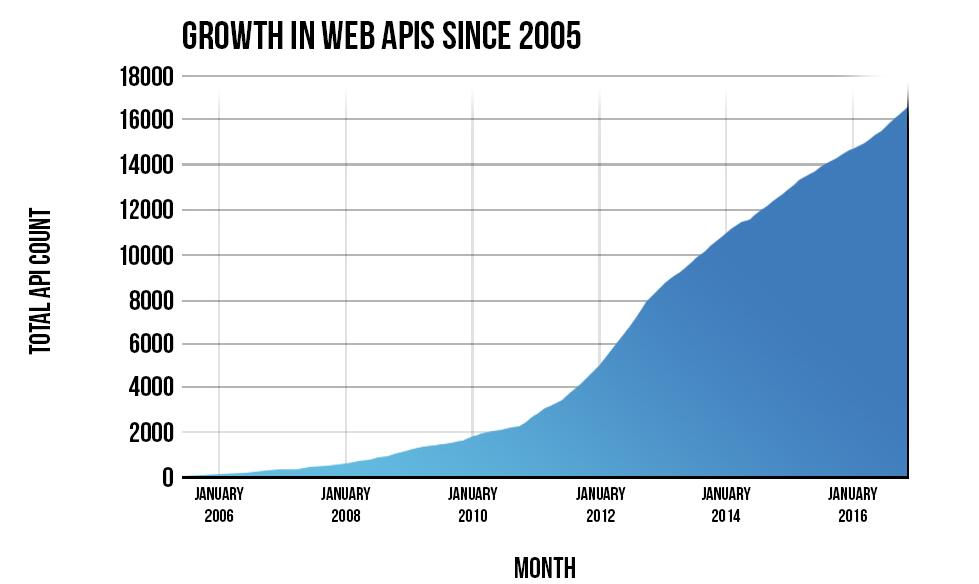
\includegraphics[width=\textwidth]{Picture1-1.jpg}\\
  \caption{2005-2016年Web服务数量}\label{fig:1}
\end{figure}
面对大量的Web服务,大部分用户由于缺乏足够的经验或者能力,很难快速找到自己想要的Web服务,这就造成了信息过载\cite{Borchers1998Ganging}问题。解决信息过载问题主要手段有两个,搜索引擎和推荐\cite{Jannach2010Recommender}。搜索引擎通过排序算法对网页进行排序,在用户进行查询时,根据用户查询的关键字,将和关键字最为相关的网页链接排序显示给用户。搜索引擎需要用户事先知道自己的需求并键入关键词,当用户不能准确描述自己需求的时候,搜索引擎便无能无力了。推荐系统的出现很好的弥补了搜索引擎这方面的不足,推荐系统不需要用户提供明确的需求,而是通过用户的历史行为给用户的兴趣建模,从而发掘出用户潜在的兴趣和需求,推荐出用户可能感兴趣的Web服务。

\section{研究现状}
随着Web服务数量的飞速增长,Web服务推荐问题吸引了越来越多的人研究,逐渐成为服务计算领域的一大热门。当前Web服务推荐研究主要分为两类,为用户推荐可能感兴趣的Web服务和为Mashup应用推荐可以满足其功能需求的Web服务API,本文主要研究的问题是为用户推荐Web服务,所以对为Mashup推荐Web服务API的研究不作阐述。目前,相关研究大多是依据用户对Web服务的历史偏好信息或者是服务本身的QoS信息,通过协同过滤(Collaborative Filtering)技术来进行推荐。下面将主要介绍基于用户历史信息的推荐以及基于服务质量QoS的推荐的相关研究现状。

基于用户历史偏好信息的推荐,首先需要收集大量用户对Web服务的历史评分信息,综合用户特征或者服务特征,找出相似的用户或者相似的服务,并以此来预测用户可能感兴趣的服务,从而个性化地为用户进行推荐。文献\cite{Ling2014Web}综合了用户特征和用户评价的相似性,通过对用户情境聚类,对结果进行过滤,实现了满足用户个性化需求的推荐。文献\cite{Zheng2009WSRec}\cite{Jiang2011An}采用了基于邻域(Neighbour-Based)的协同过滤方法,在计算用户或者服务相似度的时候,考虑了不同用户和服务的个性化的特征,最后通过最相近的$k$个用户或者服务的评分来预测评分。文献\cite{Tian2014Time}提出了一种时间感知的Web服务推荐方法,通过对用户评分习惯随时间变化而变化,服务的热门程度随时间变化而变化,用户对服务的评分随时间变化而变化这三种场景进行建模,并结合矩阵分解方法进行评分预测。当前,这些方法主要的问题是,只考虑了用户的历史偏好信息,而忽视了Web服务丰富的边缘信息\cite{Shi2014Collaborative}。

基于QoS的服务推荐,通过收集大量的用户调用Web服务时的QoS信息,例如响应时间、吞吐率、价格成本等等\cite{Qi2010Combining},使用协同过滤技术预测QoS值,再根据预测的QoS值来进行推荐\cite{Zheng2011QoS}。文献\cite{Shao2007Personalized}认为相似的用户倾向于接受拥有相似QoS值的Web服务,并基于这一假设提出了一种基于用户的(User-Based)的协同过滤方法来预测Web服务的QoS值。文献\cite{Zheng2013Collaborative}使用矩阵分解技术来预测Web服务的QoS值,取得了比基于邻域的协同过滤方法更好的准确度。为了提高QoS预测的准确性,有不少工作考虑在推荐模型中添加一些额外的信息,例如地点位置信息,用户的历史调用记录,以及时间信息等。文献\cite{Zhang2011Collaborative}使用用户的历史调用信息来推断用户的行为特征,通过历史调用信息来计算用户之间的相似度,并将相似度与协同过滤方法相结合以计算QoS的值。文献\cite{conf/icws/TangJLL12}将地理位置信息引入到了Web服务推荐,将用户和服务按照地理位置进行划分,根据地理位置信息来寻找相似的用户或者相似的服务,从而通过协同过滤方法来预测缺失的QoS值。文献\cite{Amin2012An}认为QoS的属性值随着时间的变化而具有波动性,文章提出了一种整合自回归积分滑动平均模型ARIMA(Autoregressive Integrated Moving Average Model)和自回归条件异方差模型GARCH(Autoregressive Conditional Heteroskedasticity Model)模型的预测方法,以便能够捕捉QoS属性的波动性并提供准确的预测。基于QoS的Web服务推荐最大的问题在于,服务的QoS的准确性往往和调用的地理位置有关,所以获取QoS信息是一件很困难的事。同时,通过QoS值来进行推荐,有时并不能有效地发掘用户的兴趣点,具有更高QoS数值的服务未必是用户感兴趣的。

\section{本文工作}
本文对当前的Web服务推荐相关工作进行了深入调研,发现目前的相关研究主要存在三个问题:(1)大量工作基于QoS进行推荐,而基于用户的历史偏好进行推荐的工作则比较少,而用户的历史偏好往往更能反映用户的兴趣,尤其是对于ProgrammableWeb网站的用户。(2)服务推荐中丰富的边缘信息没有能够很好的利用起来,例如功能主题信息和服务组合信息,这些边缘信息蕴含了Web服务在功能和结构上的联系,可以弥补用户历史偏好信息的稀疏性,对推荐准确性的提升很有帮助。(3)当前的Web服务推荐相关工作,在评估指标上往往只关注准确性,而忽视了推荐结果的多样性。针对当前工作中存在的以上问题,本文基于服务平台ProgrammableWeb网站的用户数据,在推荐的准确性和多样性方面作了如下工作:
\begin{enumerate}
\item 在准确性方面,提出了一个基于主题信息和服务组合信息的Web服务推荐算法,该算法基于ProgrammableWeb网站的真实数据,通过用户的隐式反馈信息来提取用户的兴趣偏好,通过ProgrammableWeb网站的服务注册页面来提取服务的功能描述信息以及服务组合信息,以此分别计算了Web服务之间在主题以及服务组合关系上的相似度,并根据相似度获取了每个Web服务在主题和服务组合关系上的邻居Web服务集合,将其与SVD(Singular Value Decomposition)矩阵分解模型相结合,以预测用户评分,提高推荐性能。

\item 在多样性方面,针对目前服务推荐在多样性上的不足,提出了一种考虑用户偏差的改进重排名算法以提高推荐的多样性,该算法考虑了用户评分习惯差异性和用户兴趣分布差异性,并将这两种偏差结合进了阈值$T_R$的计算中,使得改进的重排名模型不再按照固定阈值$T_R$而是通过加入了用户差异性的个性化阈值来为用户提高多样性。实验表明,与经典的重排名算法\cite{Adomavicius2009TOWARD}相比,该算法可以在尽量少地牺牲准确性的基础上,尽量多地提高Web服务推荐的多样性。

\item 使用ProgrammableWeb网站的真实数据作为数据集,其中包括超过280000个用户服务交互记录,65000服务用户和15000个Web服务或Mashup。基于该数据集进行了一系列的实验,以验证我们方法的有效性。
\end{enumerate}



\section{本文组织}
本篇论文主要由五个章节组成,第一章作为全文的绪论,阐述了论文的研究背景,相关工作的研究现状,本文的主要工作和内容章节安排。论文的其他四章内容如下:

第二章主要介绍与本文研究内容相关的工作和技术,主要包括Web服务推荐的研究现状和挑战,Web服务推荐中常用的技术和评估方式以及推荐多样性的提高算法,为后续章节作好铺垫。

第三章主要介绍融合主题信息和服务组合信息的Web服务推荐算法,首先给出了算法的提出动机,然后介绍了用户评分信息的计算,服务功能主题信息相似度和服务组合相似度的计算以及与矩阵分解模型的融合,最后通过实验验证了我们算法的有效性。

第四章首先介绍了Web服务多样性的提出动机,然后介绍了用户评分的获取以及用户偏差的定义和表示,并在考虑用户偏差的基础上提出了一种改进的重排名算法,最后通过实验验证了我们算法的有效性。

第五章是对全文工作的总结,并对未来的研究工作进行展望。

\chapter{相关工作和技术}\label{chapter_relatework}
\section{Web服务推荐}
随着互联网上Web服务数量的增加,如何向用户推荐合适的服务成为了一大问题。Web服务推荐是帮助用户发现合适服务的有效手段之一,近年来逐渐成为服务计算领域的研究热点。Web服务的一般过程是,首先收集用户的基本信息、历史调用记录、服务的相关信息,然后建立推荐预测模型,最后根据模型预测用户可能感兴趣的Web服务进行推荐。Web服务推荐的关键就是,如何利用数据挖掘和机器学习相关技术来预测用户的需求,帮助用户发现感兴趣的Web服务。

Web服务推荐系统的框架如图\ref{2-1}所示,通常包括三个部分,首先对数据进行清洗、整理和转换,然后对用户、服务以及内容特征建模,最后通过推荐策略模块来产生推荐,推荐策略通常包括协同过滤、基于内容的推荐以及混合推荐。
\begin{figure}[htbp]
  \centering
  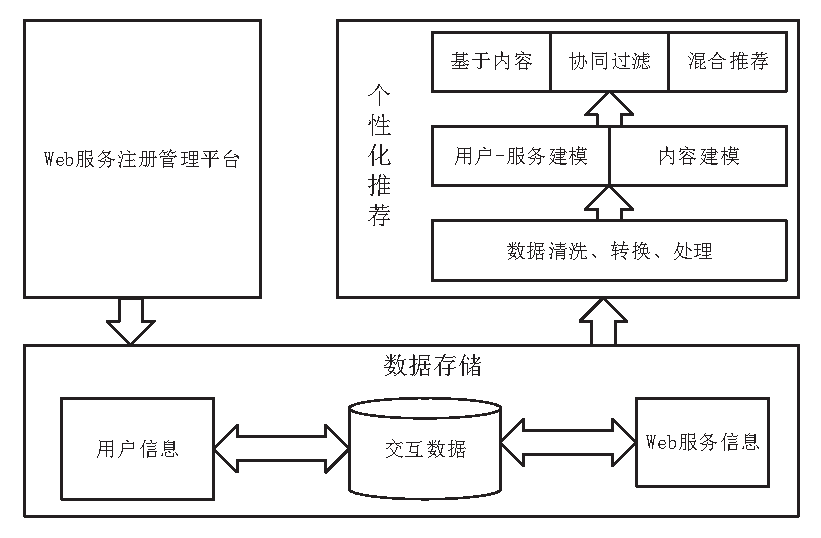
\includegraphics[width=0.9\textwidth]{2-1.eps}\\
  \caption{Web服务推荐框架}\label{2-1}
\end{figure}

目前Web服务推荐的研究主要可以分为以下几类:
\begin{enumerate}
\item \emph{基于功能的推荐}~基于功能的推荐利用自然语言处理的相关技术,通过挖掘Web服务的功能信息,来找到那些功能相似的Web服务。文献\cite{Dong2004Similarity}利用关键词提取来进行语义匹配,文献\cite{Li2013A}利用LDA(Latent Dirichlet Allocation)主题模型从服务的WSDL描述文档中提取潜在特征。基于功能的推荐产生的推荐结果较为单一,并且Web服务的WSDL文档往往很难获得。

\item \emph{基于QoS的推荐}~基于QoS的推荐通过收集大量的用户调用Web服务时的QoS信息,例如响应时间、吞吐率、价格成本等等,使用协同过滤技术预测Web服务的QoS值,最后根据QoS值进行推荐。文献\cite{Zheng2013Collaborative}使用矩阵分解技术来预测Web服务的QoS值。文献\cite{Yao2013Recommending}将协同过滤与基于内容的推荐相结合,进一步提升了推荐的准确性。文献\cite{Qi2015Personalized}考虑了Web服务QoS值在地点上的关联性,将地理位置信息与矩阵分解模型相结合,取得了不错的效果。文献\cite{Li2017Temporal}考虑了时间对QoS的影响,通过在相似度计算中引入时间信息来提高QoS的预测效果。基于QoS的推荐的主要问题是,服务的QoS信息往往与调用的地理位置有关,通常很难获取服务准确的QoS值。

\item \emph{基于历史偏好信息的推荐}~基于历史偏好信息的Web服务推荐,需要从服务发布平台上收集大量的用户显式或者隐式评分信息、用户或者服务的特征信息,综合这些信息利用相关推荐技术进行推荐。文献\cite{Gao2016Joint}考虑了Mashup在服务推荐中的作用,利用图模型来构建用户、服务以及Mashup之间的关系,从而完成推荐。文献\cite{Tian2014Time}提出了一种时间感知的Web服务推荐方法,并结合矩阵分解模型进行评分预测。文献\cite{Qi2017Data}将用户的社交关系信息与协同过滤方法相结合,并通过剪枝策略来缩减搜索空间,有效地减小了数据稀疏性带来的影响,提升了预测准确性。文献\cite{Zhang2017Recommendation}提出了一种“分而治之”的方法,通过将标签信息与协同过滤相结合,着重对新加入的Web服务进行推荐。基于历史偏好信息的推荐的主要问题是,用户的偏好信息通常比较稀疏,如何解决数据的稀疏性问题是关键。

\end{enumerate}

当前,Web服务推荐仍然面临很多挑战,主要有以下几点:
\begin{enumerate}
\item \emph{数据稀疏性}~Web服务推荐需要利用用户的历史数据来发掘用户兴趣,然而QoS数据由于其通常跟地点有关,具有不稳定性,导致用户真实的QoS数据往往难于收集。而用户使用过的服务,通常相对于服务发布平台上的大量服务来说数量过于稀少,这也导致了基于用户历史偏好信息来进行Web服务推荐同样面临数据的稀疏性问题。

\item \emph{服务的异构性}~对于不同类型的Web服务,很难用统一的方式进行建模或者特征提取,根据ProgrammableWeb的统计,发布在该网站上的遵循SOAP协议的Web服务约占21$\%$,遵循REST协议的轻量级RESTful服务约占70$\%$,Web服务间的异构性大大增加了服务推荐的难度。

\end{enumerate}

针对Web服务推荐的研究现状和挑战,本文基于ProgrammableWeb网站来提取用户的历史偏好信息,利用网站上统一的描述信息来取代Web服务传统的WSDL描述文档,通过提取网站上丰富的边缘信息来弥补数据稀疏性。

\section{Web服务推荐中的推荐技术}
自20世纪90年中期出现了第一批关于协同过滤的文章\cite{Hill:1995:REC:223904.223929,resnick94:_grouplens}以来,推荐技术逐渐成为热门的研究领域。服务推荐中常用的推荐算法有三种:基于协同过滤的推荐、基于内容(Content-Based)的推荐以及混合了内容与协同过滤的推荐,而基于协同过滤的推荐算法又可以分为基于邻域的推荐和基于模型(Model-Based)的推荐。图\ref{fig:2}展示了推荐算法的分类框架,下面将分别对这些方法进行介绍。
\begin{figure}[htbp]
  \centering
  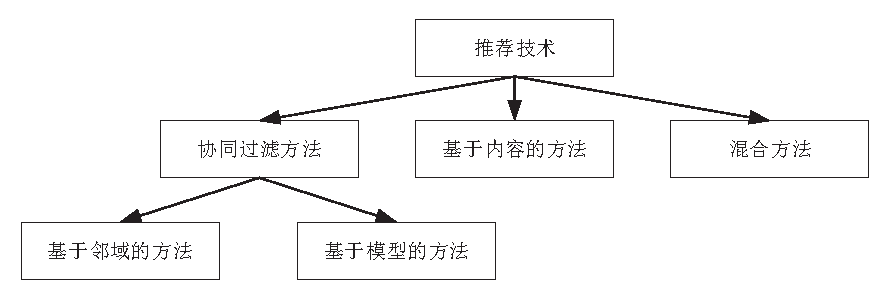
\includegraphics[width=\textwidth]{CF1.eps}\\
  \caption{推荐算法分类}\label{fig:2}
\end{figure}

\subsection{协同过滤}
协同过滤技术通过用户对项目的历史偏好信息来发掘用户或者项目之间的相关性,再根据这些相关性来进行推荐。目前,基于协同过滤的推荐系统在工业界得到了广泛的应用,包括新闻推荐系统GroupLens\cite{resnick94:_grouplens}、视频推荐系统Video Recommender\cite{Hill:1995:REC:223904.223929}、书本推荐系统Amazon.com\cite{Linden-Amazon-2003}。

协同过滤算法通常被分为两类,基于邻域的协同过滤算法和基于模型的协同过滤算法,下面对这两类算法进行介绍,为了方便描述,表\ref{table:1}给出了后面可能用到的符号说明。
\begin{table}
  \centering
  \begin{tabular}{|c|c|}
    \hline
    \textbf{符号} & \textbf{说明} \\
    \hline U  & 用户集 \\
    \hline I     &项目集   \\
    \hline $M$  & 用户的总数\\
    \hline  $N$   & 项目的总数     \\
	\hline  $T$   &测试集    \\
	\hline   $r_{ui}$  & 用户$u$对项目$i$的真实评分     \\
	\hline   $\hat{r}_{ui}$ & 用户$u$对项目$i$的预测评分     \\
	\hline    $I_u$ &用户$u$评价过的项目集合    \\
	\hline    $L_u$ &用户$u$的推荐列表    \\
	\hline    $B_u$ & 测试集中用户$u$选择的项目集合     \\
	\hline    $p_i$ & 项目$i$的度,即评价过项目$i$的用户数量\\
	\hline    $N(u)$ &用户$u$的邻居集合\\
    \hline
  \end{tabular}
  \caption{符号说明表}\label{table:1}
\end{table}

\begin{enumerate}
\item \emph{基于邻域的协同过滤算法}~基于邻域的协同过滤算法可以分为基于用户的协同过滤和基于项目(Item-Based)的协同过滤。基于邻域的协同过滤算法主要有以下三个过程:
\begin{enumerate}
\item \emph{建立用户-项目矩阵}~首先需要收集用户的各种历史偏好信息,例如用户对项目的评分信息,建立用户-项目矩阵。如图\ref{fig:3}所示,给定一个包含$M$个用户和$N$个项目的推荐系统,我们建立一个$M\times N$的用户-项目矩阵,其中矩阵中的项$r_{ui}$表示用户$u$对项目$i$的评分值,如果$r_{ui}$值不存在,说明用户$u$从未对项目$i$评价过。
\begin{figure}[htbp]
  \centering
  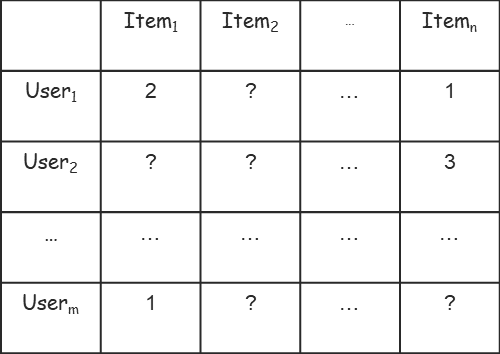
\includegraphics[width=0.6\textwidth]{User-item-matrix.png}\\
  \caption{用户-项目矩阵}\label{fig:3}
\end{figure}
\item \emph{计算用户或者项目之间的相似度}~需要寻找那些相似的用户或者相似的项目,这一步的关键是根据用户-项目矩阵,计算物品或项目之间的相似度。常用的相似度计算方法有余弦相似度\cite{Breese1998Empirical}和皮尔逊相关系数PCC(Pearson Correlation Coefficient)。以基于用户的协同过滤为例,可以通过皮尔逊相关系数来定义用户$u$和用户$v$之间的相似度$Sim(u,v)$如下:
\begin{equation}
Sim(u,v)=\frac{\sum\limits_{i\in I_{u}\bigcap I_{v}}(r_{u,i}-\bar{r_{u}})(r_{v,i}-\bar{r_{v}})}{\sqrt{\sum\limits_{i\in I_{u}\bigcap I_{v}}(r_{u,i}-\bar{r_{u}})^{2}}\sqrt{\sum\limits_{i\in I_{u}\bigcap I_{v}}(r_{v,i}-\bar{r_{v}})^{2}}}
\end{equation}
其中,$\bar{r_{u}}$、$\bar{r_{v}}$分别表示用户$u$、$v$对他们共同评价过的项目集合 $I_{u}\bigcap I_{v}$中的各项目评分的平均值。$Sim(u,v)$的值在-1和1之间,值越大表明用户$u$和$v$之间越相似。在基于用户的协同过滤中,也可以用余弦相似度来定义用户$u$和用户$v$之间的相似度$Sim(u,v)$,定义如下:
\begin{equation}
Sim(u,v)=\cos(\vec{u},\vec{v}) =\frac{\vec{u}\cdot \vec{v}}{\left \| \vec{u} \right \|\times \left \| \vec{v} \right \|}=\frac{\sum\limits_{i\in I_{u}\bigcap I_{v}}r_{u,i}r_{v,i}}{\sqrt{\sum\limits_{i\in I_{u}\bigcap I_{v}}r_{u,i}^{2}}\sqrt{\sum\limits_{i\in I_{u}\bigcap I_{v}}r_{v,i}^{2}}}
\end{equation}
$Sim(u,v)$的取值在$[0,1]$,值越大表明用户$u$和$v$越相似。

\item \emph{通过最相似的若干邻居评分预测用户评分,产生推荐结果}~在有了用户或者项目之间的相似度之后,需要通过若干邻居的聚合来预测评分,常用的预测如下:
\begin{equation}
\hat{r}_{ui}=\frac{\sum\limits_{{u}'\in N(u)}Sim(u,{u}')r_{{u}'i}}{\sum\limits_{{u}'\in N(u)}\left | Sim(u,{u}') \right |}
\end{equation}
\end{enumerate}
基于邻域的协同过滤方法的结果可解释性很强,这在推荐系统中是一个很重要的方面。同时,算法简单易于实现,具有很强的扩展性。但是当数据变得稀疏时,相似度的计算会不准确,算法的性能会极大地下降。

\item \emph{基于模型的协同过滤算法}~基于模型的协同过滤方法从用户的历史评分信息中学习出一个预测模型,然后通过这个模型进行评分预测。模型的学习通常需要借助机器学习的方法。常用的模型有贝叶斯网络、聚类模型、潜在语义模型、矩阵分解模型、马尔科夫模型等。下面重点介绍一下矩阵分解模型。

矩阵分解模型将用户的评分信息映射到一个低维的隐向量空间,用户对项目的评分可以表示成两个向量的内积。通常项目$i$表示为向量$q_i\in\mathbb{R}^f$,向量$q_i$的元素表示了项目$i$具有这些隐因子的丰富程度,每个用户$u$表示为向量$p_u\in\mathbb{R}^f$,向量$p_u$表示用户对各个隐因子的兴趣。用户的评分估计可以表示为这两个向量的乘积:
\begin{equation}
\hat{r}_{ui}=q_i^Tp_u\label{eq:mf}
\end{equation}
矩阵分解所要做的,就是计算用户和项目到隐向量的映射,即找到两个矩阵$P$、$Q$,它们相乘之后得到的值,和待分解矩阵中有值的位置中的值尽可能地接近,这样一来分解出来的两个矩阵相乘就尽可能地还原了待分解矩阵,因为有值的地方,值都相差得尽可能地小,那么没有值的地方,通过这样的方式算出的值,也就比较符合趋势。对每个用户$u$和项目$i$,找到这样的$p_u$和$q_i$,满足如下目标函数:
\begin{equation}
\min_{q, p}\sum_{(u,i)\in\mathcal{R}}(r_{ui}-q_i^Tp_u)^2 
\end{equation}
其中$\mathcal{R}$是用户对项目的历史评分集合。通常,为了防止过拟合,会在上式中加入正则项,加入正则项后的目标函数如下:
\begin{equation}
\min_{q, p}\sum_{(u,i)\in\mathcal{R}}(r_{ui}-q_i^Tp_u)^2 + \lambda(\|p_u\|^2 + \|q_i\|^2)
\end{equation}
其中$\lambda$是正则项系数,用于控制正则化的程度。求解上面的目标函数,通常采用随机梯度下降的方法。首先对于每个用户-项目评分,计算预测误差$e_{ui}$:
\begin{equation}
e_{ui} = r_{ui} - q_i^Tp_u
\end{equation}
然后按照梯度下降的方向更新用户和项目的隐向量,直到算法收敛或者到达给定的迭代数。
\begin{equation}
q_i \leftarrow q_i + \gamma\cdot(e_{ui}\cdot p_{u}-\lambda\cdot q_i)
\end{equation}
\begin{equation}
p_u \leftarrow p_u + \gamma\cdot(e_{ui}\cdot q_{i}-\lambda\cdot p_u)
\end{equation}
其中$\gamma$是学习率,用于控制算法收敛的速度。对于任意用户$u$以及任意项目$i$,我们即可通过公式\eqref{eq:mf}计算得到的$p_u$和$q_i$来估算用户的评分$\hat{r}_{ui}$。

基于模型的协同过滤算法相比基于邻域的协同过滤算法,能够更好地解决原始矩阵的稀疏性问题,特别在处理大型稀疏数据集时。但是模型的训练通常需要大量时间,并且对于推荐项目的可解释性不如基于邻域的协同过滤。
\end{enumerate}

\subsection{基于内容的推荐}
基于内容的推荐算法的思想很简单,就是根据用户过去喜欢的项目,为用户推荐和他们过去喜欢的项目相似的项目。基于内容的推荐不依赖于用户对项目的评价,而是更多地对项目的内容和用户的兴趣进行匹配,再推荐那些项目内容与用户兴趣相似度高的其他项目。

基于内容的推荐系统通常包含三个部分:用户特征提取、项目特征提取、生成推荐列表,如图\ref{fig:4}所示。用户特征提取,即利用一个用户过去喜欢(及不喜欢)的项目的特征数据,来学习出此用户的喜好特征。项目特征提取,即为每个项目抽取一些特征来表示这个项目。生成推荐列表,即通过将用户喜好特征与候选项目的特征进行比较,为此用户选择一组相关性最大的项目。
\begin{figure}[htbp]
  \centering
  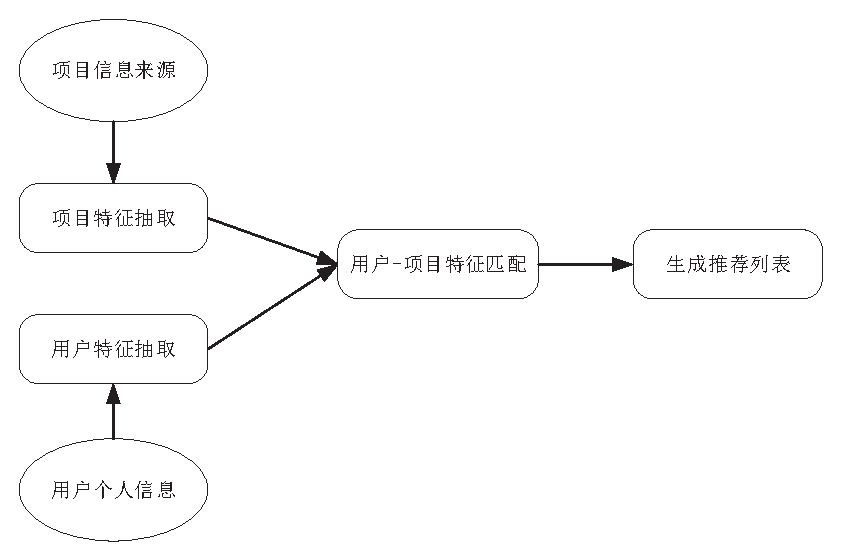
\includegraphics[width=0.8\textwidth]{Content_based.eps}\\
  \caption{基于内容的推荐系统流程}\label{fig:4}
\end{figure}

在基于内容的推荐中,常常采用LDA(Latent Dirichlet Allocation)\cite{Blei2003Latent}主题模型来进行特征提取,下面我们将对LDA主题模型进行简要介绍。我们先介绍一下什么是主题。主题是对文本内容的一个提炼,当我们读一篇文章时,可能会想概括一下这篇文章主要讲什么,此时我们可能会回答,80\%在讲政治,15\%在讲娱乐,其余在讲废话,那么我们就可以从这篇文章提炼出三个主题:政治、娱乐、废话。那么我们又是怎么提炼出一篇文章的主题呢?我们通常是因为一篇文章出现了某些特定的词,而这些词往往和某个特定的主题想关联, 所以通过这些词就可以确定某一篇文章的主题。以表\ref{topic_table}为例,我们在文本中出现了诸如``Film",``Music",``Show"等关键词,所以我们通过这些词归纳出``Arts"这一主题。同理,我们根据文本中的其他词,将文本归纳为了四个主题,分别``Arts",``Budgets",``Children",``Education",每个主题下会有能体现该主题特征的关键词。
\begin{table}[htbp]
\centering
\caption{一个主题和关键词的例子}
\label{topic_table}
\begin{tabular}{llll}
\hline
``Arts"  & ``Budgets" & ``Children" & ``Education" \\ \hline
NEW     & MILLION   & CHILDREN   & SCHOOL      \\
FILM    & TAX       & WOMEN      & STUDENTS    \\
SHOW    & PROGRAM   & PEOPLE     & SCHOOLS     \\
MUSIC   & BUDGET    & CHILD      & EDUCATION   \\
MOVIE   & BILLION   & YEARS      & TEACHERS    \\
PLAY    & FEDERAL   & FAMILIES   & HIGH        \\
MUSICAL & YEAR      & WORK       & PUBLIC      \\
BEST    & SPENDING  & PARENTS    & TEACHER     \\
ACTOR   & NEW       & SYAS       & BENNETT     \\
FIRST   & STATE     & FAMILY     & MANIGAT     \\
YORK    & PLAN      & WELFARE    & NAMPHY     
\end{tabular}
\end{table}

LDA主题模型由David M.Blei和Michael I.Jordan在2003年提出,是一种的非监督的概率生成模型,可以用来发现文档的隐含主题。LDA认为一篇文章的每个词都是由一个生成过程得到的,即文章以一定的概率选择了某一个主题,某个主题又以一定的概率选择了某一个词。对于语料库中的文档,LDA模型生成过程如下:
\begin{arabicenum}
\item 从狄利克雷分布 $\alpha$ 中取样生成文档$i$的主题分布 $\theta_{i}$
\item 从主题的多项式分布$\theta_{i}$中取样生成文档$i$第$j$个词的主题 $z_{ij}$
\item 从狄利克雷分布$\beta$中取样生成主题$z_{{ij}}$的词语分布$\phi_{z_{ij}}$
\item 从词语的多项式分布$\phi_{z_{ij}}$中采样最终生成词语$w_{ij}$
\end{arabicenum}
上述生成过程可以用图\ref{fig:11}表示。
\begin{figure}[htbp]
  \centering
  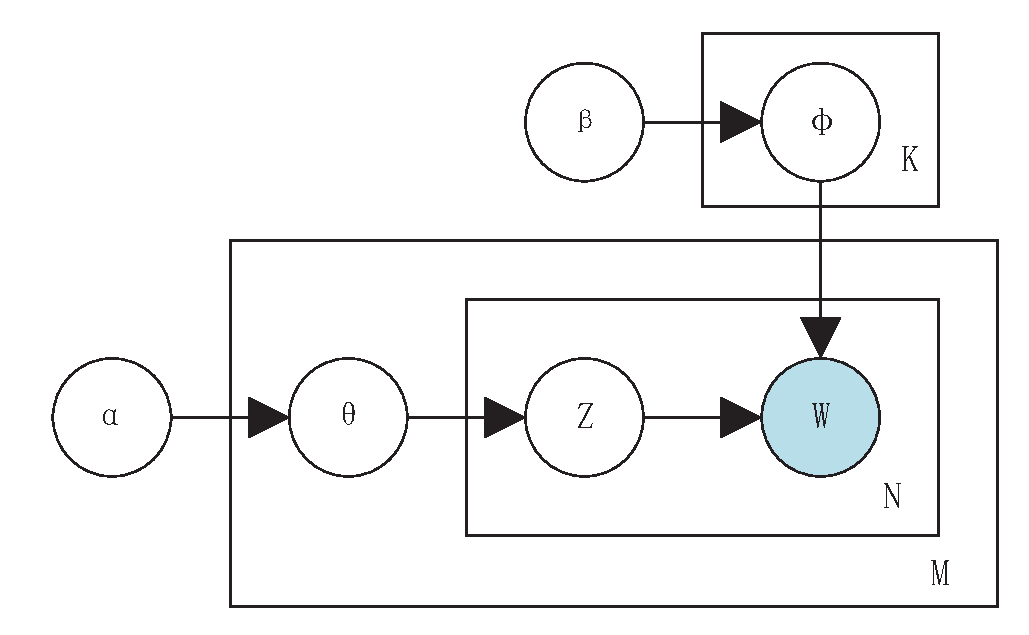
\includegraphics[width=0.5\textwidth]{LDA.eps}\\
  \caption{LDA模型生成概率图}\label{fig:11}
\end{figure}

LDA模型有两个分布参数需要学习:一个是文档-主题(Document-Topic)分布$\theta$,一个是主题-词(Topic-Word)分布$\phi$。这两个参数可以通过Gibbs采样来估计得到,这里不再赘述,详细过程可参考文献\cite{Heinrich2008Parameter}。最终,$\theta$和$\phi$的估计公式如下:
\begin{equation}
\phi _{{k,t}}=(n_{k}^{{(t)}}+\beta _{t})/(n_{k}+\beta _{t})
\end{equation}
\begin{equation}
\theta _{{m,k}}=(n_{m}^{{(k)}}+\alpha _{k})/(n_{m}+\alpha _{k})
\end{equation}
其中,$n_{k}^{{(t)}}$表示词汇$t$属于主题$k$的次数,$n_{k}$主题$k$中的词汇总频数,$n_{m}^{{(k)}}$表示第$m$篇文章中主题$k$出现的次数,$n_{m}$表示第$m$篇文章的主题出现总频数。

基于内容的推荐过程简单可解释性强,推荐的结果容易被人接受,对于没有任何用户评分的新项目,也可以推荐给用户。但是基于内容的推荐也有一定的局限性:(1)可分析的内容有限,无法区分具有相同特征的不同项的质量。(2)推荐的项目没有很好的新颖性,不能为用户发现一些新的潜在的感兴趣的项目。

\section{推荐算法的评估方式}
推荐算法的研究中,如何评价一个推荐算法的好坏是一个不可忽视的问题。当前很多工作对推荐系统的评估指标进行了研究,文献\cite{Sarwar2001Item,朱郁筱2012推荐系统评价指标综述}在对推荐系统的评估方法进行了总结,它将评估方法分为在线评估、用户调查和离线评估。由于用户调查和在线评估都需要大量用户的参与,评估代价较高,目前大多数研究主要采用的都是离线评估。文献\cite{朱郁筱2012推荐系统评价指标综述}对离线评价中常用的指标进行了总结,包括准确性指标和非准确性指标,准确性指标包括准确率、召回率,F-Measure、均方根误差(RMSE)等,非准确性指标包括多样性、新颖度、覆盖率等指标,下面将对重点介绍准确性指标和多样性指标。

\subsection{准确性指标}
预测的准确性是推荐系统研究中讨论最多的属性,推荐系统有一个最基本的假设,即用户更喜欢推荐更精确的系统,因此大量国内外研究人员都致力于寻找更精确的预测算法。通常算法的准确性指标分为两大类,评分预测准确性和使用预测准确性。

\begin{enumerate} 

\item \emph{评分预测准确性}~在一些推荐系统中,我们的核心任务就是预测用户对某个物品的评分(如1到5分)。在这种情况下,我们可以通过评分预测准确性指标来评估推荐系统。在评分预测准确性指标中,均方根误差和平均绝对误差(MAE)是最常用的度量指标,它们体现了真实评分和预测评分之间的差异性大小,通常RMSE和MAE的值越小,预测的准确性越高。

均方根误差定义如下:

\begin{equation}
RMSE=\sqrt{\frac{1}{\left | T \right |}\sum_{(u,i)\in T}(r_{ui}-\hat{r}_{ui})^2 }
\end{equation}

平均绝对误差定义如下:

\begin{equation}
MAE=\frac{1}{\left | T \right |}\sum_{(u,i)\in T}\left | r_{ui}-\hat{r}_{ui} \right |
\end{equation}

\item \emph{使用预测准确性}~在很多推荐系统中,推荐系统并不预测用户的偏好(如电影评分),而是预测用户可能会喜欢的项目,在这种情况下,我们并不关心推荐系统是否正确地预测了用户的评分,而更关心推荐的项目是否被添加到了用户喜欢的列表中。我们可以通过使用准确性指标来评估这类推荐系统。常用的使用预测准确性指标包括精度(Precision)、召回率(Recall)等。

精度表示推荐给用户的项目中,用户喜欢的项目所占的比例,单个用户$u$推荐精度如下:

\begin{equation}
Precision(L_u)=\frac{\left |L_u\bigcap B_u \right |}{\left | L_u \right |}
\end{equation}

召回率表示用户喜欢的项目中,有多少比例是推荐系统推荐给用户的,召回率通常表示如下:

\begin{equation}
Recall(L_u)=\frac{\left |L_u\bigcap B_u \right |}{\left | B_u \right |}
\end{equation}

\end{enumerate}
\subsection{多样性指标}
推荐系统的评估中,只考虑准确性指标有时是不够的,“准确”的推荐有时并不能让用户满意,有时候还必须让推荐的项目更加多种多样,因此在评估推荐系统时,讨论推荐的多样性也是有必要的。推荐的多样性指标主要分为两种,分别是个体多样性和总体多样性。个体多样性是指对单个用户而言推荐的项目是多种多样的,而总体多样性是指对于全体用户,系统推荐的项目是多样的。

个体多样性\cite{Jannach2010Recommender}通常用推荐给用户的项目中项目的平均相似度来表示,平均相似度越高,多样性往往越低。通常推荐的多样性表示如下:
\begin{equation}
Diversity(L_u) = \frac{2\sum_{i,j\in L_u,i\neq j}similarity(i,j)}{\left | L_u \right |(\left | L_u \right |-1)}
\end{equation}
其中$similarity(i,j)$表示项目$i$和项目$j$之间的相似度,相似度的计算可以参考上一节。

文献\cite{Weng2007Improving}通过新颖度来衡量推荐算法的多样性,新颖度表示推荐给用户那些该用户从未听说过的项目的能力,在新颖度评估时通常基于这样的一个假设,即流行度越低的物品往往对用户来说是越新颖的,所以通常通过平均流行度来表示推荐的新颖度,表示如下:
\begin{equation}
Novelty(L_u) = \frac{2\sum_{i\in L_u}p_i}{\left | L_u \right |}
\end{equation}
整个系统的新颖度可以表示为:
\begin{equation}
Novelty = \frac{1}{M}\sum_{u \in U}Novelty(L_u)
\end{equation}


总体多样性方面,通常使用推荐给所有用户的不同项目总数来衡量,称之为diversity-in-top-N,可以表示如下:
\begin{equation}
diversity-in-top-N=\left | \bigcup_{u \in U}L_u \right |
\end{equation}



\section{基于重排名的多样性提高算法}

推荐的多样性由Smyth Barry等人在2001年\cite{Smyth2001Similarity}首次提出,多样性表明一个推荐系统应该包含多种多样的项目,因为用户的兴趣是广泛的,只推荐用户热门的项目或者单一种类的项目虽然有可能取得较高的推荐准确性,但是往往不能令用户满意\cite{Zhou2010Solving},因为有时盲目崇拜精确性指标可能会导致用户得到一些信息量为0的“精准推荐”,使得用户视野变得越来越窄\cite{Mcnee2006Being}。

推荐系统通常包含评分预测和推荐列表生成两大步骤,评分预测即根据用户的历史偏好信息预测用户对项目的评分,而列表生成则是根据预测评分,选择评分最高的N个项目推荐给用户。因此,多样性提高算法也可以分为两类:第一类是在评分预测阶段进行\cite{Park2008The,Singh2016Relative,Yin2012Challenging},通过考虑各种综合因素来产生多样化的预测评分。第二类是在列表生成阶段进行\cite{Adomavicius2012Improving,article2011,汪千松2017一种基于参数化重排名提高多样性的推荐方法},这种方法在已有的评分预测模型的基础上,通过对推荐列表按照一定的原则来重新排序,从而提高推荐列表的多样性。与第一类方法相比,第二类方法具有更好的扩展性,能够和任何具有评分预测功能的推荐算法相结合。下面我们将主要介绍重排名算法。

推荐系统通过某种推荐算法为每个用户预测出未知的评分后,会将预测评分按照从高到低排序,从而选出评分最高的的$N$个项目推荐给用户。这种将预测评分降序排列的排序方法被称为标准排名法\cite{Adomavicius2009TOWARD}。标准排名法总是将具有最高预测评分的项目推荐给用户,虽然这样具有较高的推荐准确性,却不利于推荐多样性提高,因为标准排名法更容易将那些较为热门的项目推荐给用户。为了解决以上问题,文献\cite{Adomavicius2012Improving}提出了重排名方法,通过一个阈值$T_R$来平衡推荐结果的准确性和多样性。对于用户$i$和参数$T_R$,重排名函数$rank_x(i,T_R)$如下式所示:
\begin{equation}
rank_x(i,T_R) = \left\{  
             \begin{array}{lr}  
            rank_x(i) ,if \ R^*(u,i)\in \left [ T_R,T_{max} \right ] &\\  
             \alpha_u+rank_{standard}(i),if \ R^*(u,i) \in \left [ T_H,T_R \right ]&\\  
      
             \end{array}  
\right.
\end{equation}
其中,$I^*_u(T_R) =\left \{R^*(u,i)\geq T_R  \right \}$,$\alpha_u= \max \limits_{i \in I^*_u(T_R)}rank_x(i)$,$rank_{standard}(i)$按照标准排序法排序,$rank_x(i)$表示按照启发式的排名方法排序,$T_R$为调整阈值,$T_H$是判定项目是否与该用户有关的阈值,例如在5分制的评分中通常取经验值3.5。

重排名法设置了一个阈值$T_R$,当预测评分大于阈值$T_R$时,使用启发式的排名方法$rank_x$进行排序;当预测评分小于阈值$T_R$时,使用标准排名法进行排序。$\alpha_u$的值表示的落在区间$\left [ T_R,T_{max} \right ]$的项目的排名的最大值,其存在可以确保预测评分落在区间$\left [ T_R,T_{max} \right ]$的项目排名比预测评分落在区间$\left [ T_H,T_R \right ]$的项目更靠前(拥有更小的名次,更高的推荐优先级)。当$T_R$越接近$T_{max}$,预测评分高的项目越有可能被推荐,推荐的准确度也将越大;当$T_R$越接近$T_H$,重排名函数越接近启发式的排名方法,将会导致准确性下降,但是多样性提升。

文献\cite{Adomavicius2012Improving}给出了三种启发式的排名方法,分别是按照项目流行度排名,逆序排名以及随机排名。以项目流行度作为启发式的排名方法为例,重排名算法工作原理如图\ref{fig:4-1}所示,图\ref{fig:4-1}(a)是
\begin{figure}[htbp]
  \centering
  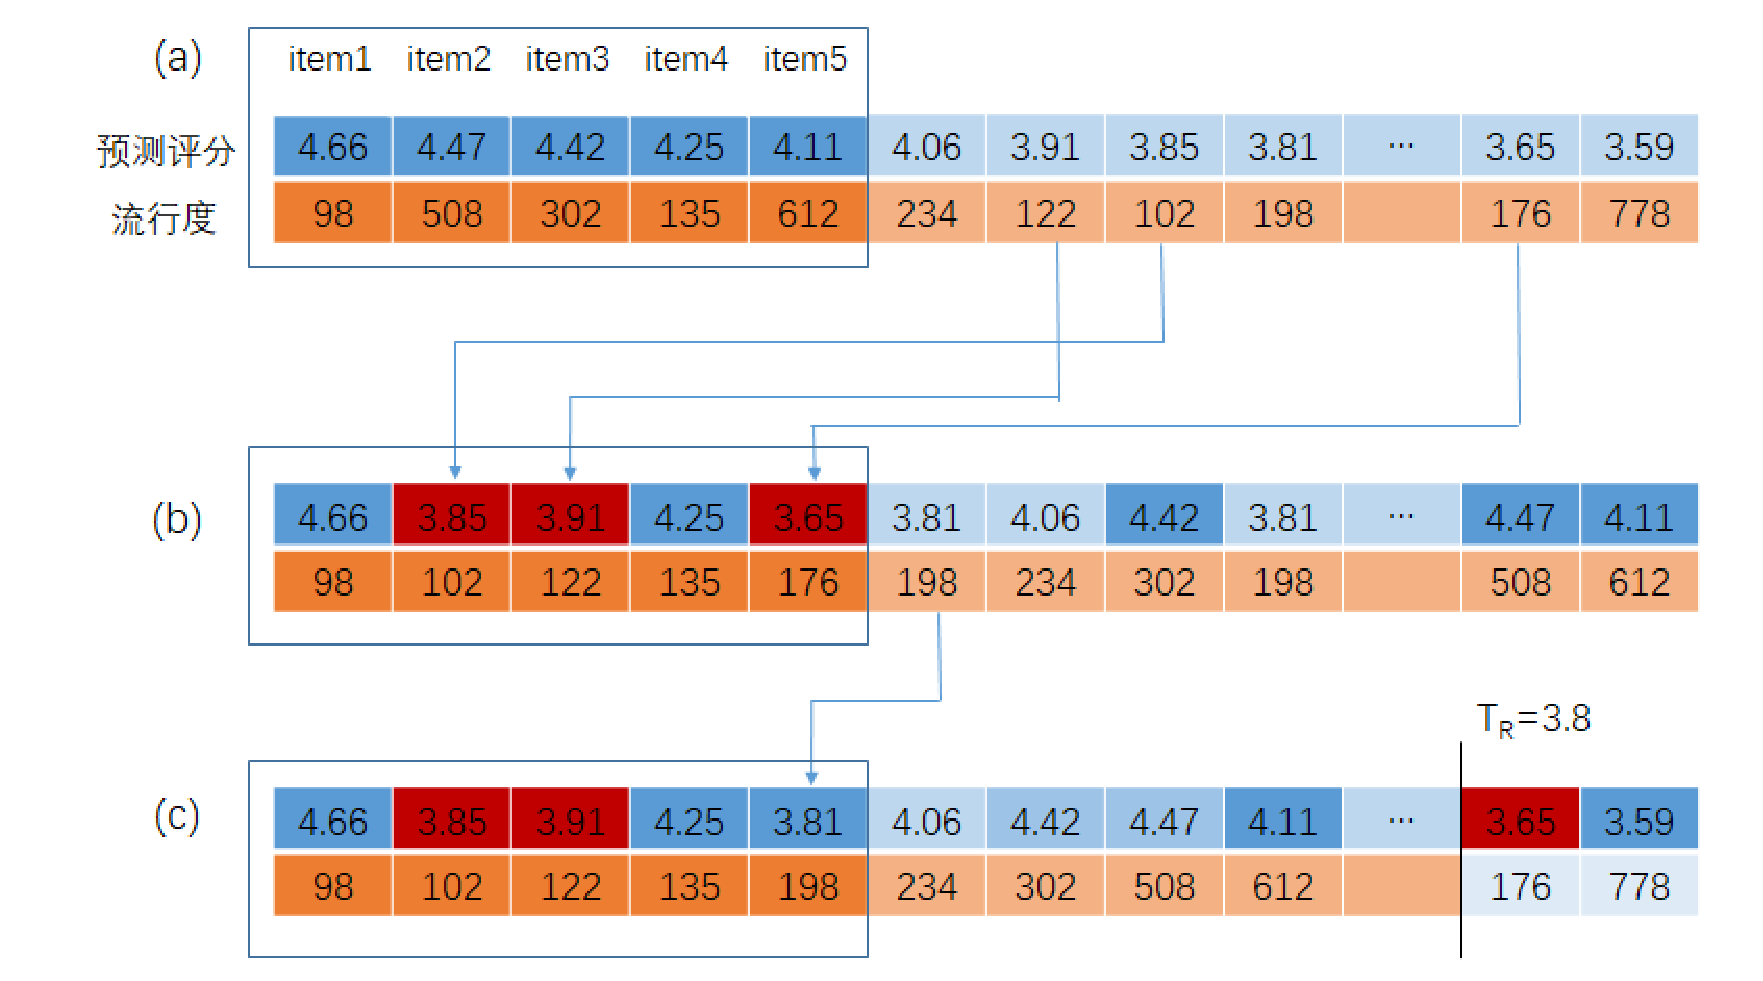
\includegraphics[width=\textwidth]{rerank_example.eps}\\
  \caption{重排名算法原理示例}\label{fig:4-1}
\end{figure}
按照标准排序法,对每个项目按照从高到低依次排序,图\ref{fig:4-1}(b)是基于项目流行度的排序方法,将与用户比较相关的项目(预测评分大于$T_H$)按照流行度从低到高排序。图\ref{fig:4-1}(c)设置阀值$T_R$为3.8,此时原预测评分为3.65的项目因为小于阈值而排名下降,而原来预测评分为3.81的项目因为流行度较低而出现在了用户的候选推荐列表中,此时推荐的准确性有所下降,但是多样性有所提升。因此通过调整阈值$T_R$,可以平衡推荐的准确性和多样性。

\section{小结}
本章首先介绍了Web服务推荐的研究现状和挑战,然后介绍了Web服务推荐中的常用技术和主要的评估方式,最后介绍了基于重排名的多样性算法,为后续章节的展开作铺垫。下面的章节将着重介绍我们的融合了主题信息和服务组合信息的Web服务推荐算法。
%%%%%%%%%%%%%%%%%%%%%%%%%%%%%%%%%%%%%%%%%%%%%%%%%%%%%%%%%%%%%%%%%%%%%%%%%%%%%%%
\chapter{融合主题信息和服务组合信息的Web服务推荐}\label{chapter_random}
\section{问题背景}
随着Web服务数量的增长,以ProgrammableWeb为代表的服务平台逐渐取代了传统的UDDI服务注册中心,成为Web服务发布、查找和使用的主要中介\cite{刘轶2016全局视角下的}。截止到2017年9月,平台上发布Web服务API的数量已达到14653,涵盖了社交、地图、搜索、天气等多个领域,而由这些Web服务组合构建而成的Mashup的数量达到了6259。经过10多年的发展,ProgrammableWeb已经成为了互联网上最大的Web服务公共平台之一。

面对如此多的Web服务,网站的用户往往会由于缺乏足够的经验或者能力,无法找到自己可能喜欢的Web服务。那么如何为网站的用户推荐他们可能喜欢的Web服务呢?当前Web服务推荐方面的研究,大多数是基于QoS的,然而对于ProgrammableWeb网站的用户来说,他们通常不关心Web服务的QoS值,他们更希望能够通过推荐发掘出他们的潜在兴趣,找到那些他们可能喜欢的Web服务。如何发掘出用户的潜在兴趣,并结合Web服务自身的一些边缘信息,来为用户推荐他们可能会喜欢的Web服务成为了一大问题。

为此,本章提出了一种融合了主题信息和服务组合信息的Web服务推荐算法,以解决以上问题。图\ref{fig:3-11}是我们的算法的框架图,主要分为评分计算、主题相似度计算、服务组合相似度计算以及模型融合等部分,下面将对这些部分进行详细介绍。
\begin{figure}[htbp]
  \centering
  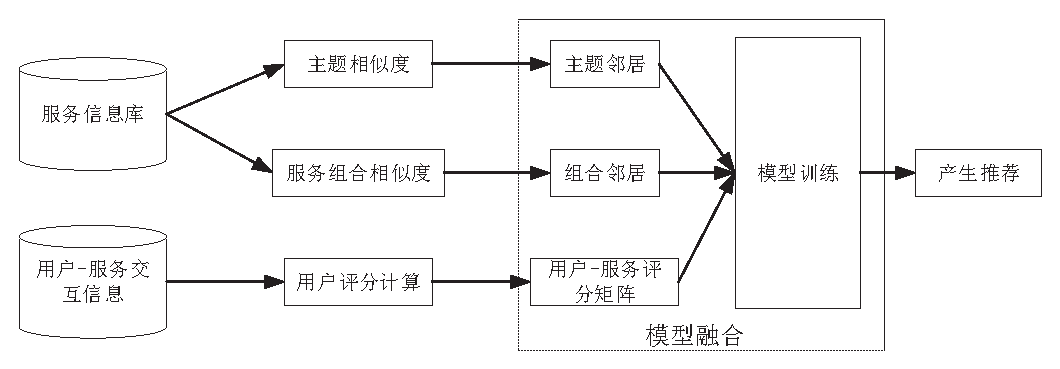
\includegraphics[width=\textwidth]{TC_SV.eps}\\
  \caption{融合主题信息和服务组合信息的Web服务推荐算法框架}\label{fig:3-11}
\end{figure}


\section{用户评分计算}
为了发掘用户的潜在兴趣,需要从用户的历史的显式或者隐式的历史记录中提取用户的偏好。然而在ProgrammableWeb上,用户的显式的评分信息很难获取, 并且很多用户往往并不会给自己喜欢的服务打一个显式的评分。为此,我们采用文献\cite{Tian2014Time}中的方法,通过用户的隐式反馈信息来提取用户的偏好\cite{Dehkordi2015Incorporating}。对于ProgrammableWeb网站的用户来说,当他们对某一个Web服务感兴趣的时候,他们可以选择“track this API”,然后这个Web服务就会被添加到该用户的观察列表(watchlist\footnote{https://www.programmableweb.com/profile/userName/alerts\#watchlist/})。通过每个用户的观察列表,我们就可以知道用户对什么样的Web服务感兴趣,从而提取用户的兴趣偏好。

进一步地,我们发现当用户的观察列表中的Web服务每次更新或者被其他用户关注以后,系统都会在该用户的观察列表中自动产生一条记录,一个Web服务被大量用户关注,说明该Web服务很受欢迎,应该具有更高的推荐的优先级,同时,我们考察一个Web服务的更新频率和该服务的受欢迎程度之间的关系,即是否经常更新的Web服务更受欢迎。我们以Google、Twitter、Yahoo和Amazon这四个知名服务提供商为例,我们统计了数据集中这四个公司更新频繁的服务和更新不频繁的服务的平均用户人数,如表\ref{table3-1}所示。
\begin{table}[h]
\centering
\caption{服务更新频率与用户数量比较表}
\label{table3-1}
\begin{tabular}{|c|c|c|c|c|}
\hline
\multirow{2}{*}{服务提供商} & \multicolumn{2}{c|}{频繁更新的服务} & \multicolumn{2}{c|}{不频繁更新的服务} \\ \cline{2-5} 
                       & 服务数量         & 平均用户数         & 服务数量          & 平均用户数         \\ \hline
Google                 & 18           & 72.8          & 103           & 22.75         \\ \hline
Twitter                & 2            & 34            & 5             & 29            \\ \hline
Yahoo                  & 5            & 48.4          & 50            & 38.14         \\ \hline
Amazon                 & 2            & 144.5         & 31            & 6.9           \\ \hline
\end{tabular}
\end{table}
以Google为例,Google提供的Web服务中,有18个更新较为频繁的服务(更新超过5次),有103个更新不太频繁的服务,对于每个频繁更新的服务,它拥有的平均用户数量是72.8,即有72.8个用户将该服务放入推荐列表中,而对于更新不频繁的服务,拥有的平均用户数量是22.75。对于Amazon,频繁更新的服务和不频繁更新的服务的平均用户数差距更大。这表明经常更新的服务更有可能受到用户的欢迎。

因此我们认为,如果用户的观察列表中某一个服务被关注或者更新的记录越多,这个服务就会更受到用户的欢迎,它应该有更高的优先级被推荐给用户,即应该具有更高的用户评分。

基于以上的阐述,我们结合用户的观察列表,给出用户的评分计算方式如下:
\begin{equation}\label{eq:3-1}
r_{us} = \frac{freq(s,Watchlist_u)+follow(s,Watchlist_u)}{Watchlist_u}
\end{equation}
其中$r_{us}$是用户$u$对服务$s$的评分,$Watchlist_u$是用户$u$的观察列表中记录总条数,$freq(s,Watchlist_u)$是用户$u$观察列表中服务$s$的更新记录条数,$follow(s,Watchlist_u)$是用户$u$观察列表中服务$s$的被用户关注记录的条数。

公式\eqref{eq:3-1}表明,当一个用户的观察列表的某个服务,更新越频繁或者关注的用户越多,该服务获得的用户评分就越高,获得的推荐优先级也越高。

我们通过公式\eqref{eq:3-1}量化了用户的兴趣偏好,为接下来的融合了主题信息和服务组合信息的Web服务推荐算法的提出作铺垫。
\section{主题相似度}
在有了用户的评分信息之后,我们便可以基于用户的历史评分信息,使用协同过滤方法进行推荐。然而,如图\ref{fig:8}所示,
\begin{figure}[htbp]
  \centering
  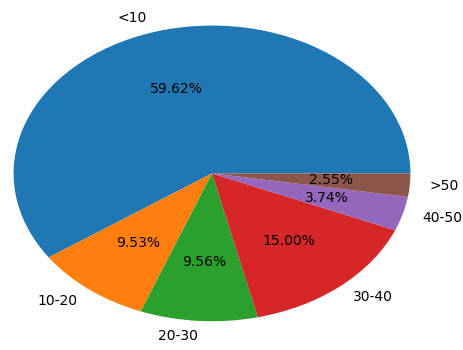
\includegraphics[width=0.5\textwidth]{pie.png}\\
  \caption{用户观察列表中Web服务数量统计}\label{fig:8}
\end{figure}
我们对数据集中的用户观察列表中的Web服务数量进行了统计,发现大约有百分之六十的用户观察列表中的Web服务数量不足10个,而观察列表中数量大于10个的用户总数加起来只有大约百分之四十,这表明在Web服务推荐中,只根据用户的观察列表进行推荐会面临着数据稀疏的问题,用户评价过的服务数与服务的总数相比太少。文献\cite{DBLP:journals/csur/ShiLH14}表明利用丰富的边缘信息可以对用户-项目矩阵进行补充,对推荐的效果有很大的帮助。为此,我们考虑充分利Web服务的边缘信息来提高推荐的性能。

大量基于内容\cite{Basu1998Recommendation,Jiang2014An,Wang2006An}的推荐研究表明,用户喜欢某一个项目,那么该用户有很大可能会喜欢跟该项目内容上相似的项目。为此,我们考虑将Web服务的功能信息融入到推荐中,如图\ref{fig:9}\footnote{https://www.programmableweb.com/mashup/segment}所示是一个Web服务在ProgrammableWeb网站中的界面,我们可以在该界面看到这个服务的名称(Name)、标签(Tags)、描述(Description)等信息。通过比较Web服务描述信息之间的语义上的相关度,我们便可以衡量两个Web服务在功能上是否相似。我们考虑通过LDA主题模型来进行文本语义的挖掘,提取Web服务的主题信息。
\begin{figure}[htbp]
  \centering
  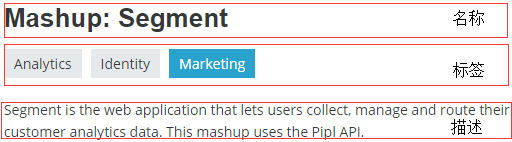
\includegraphics[width=\textwidth]{Segment.png}\\
  \caption{Segment在ProgrammableWeb中的界面}\label{fig:9}
\end{figure}
\subsection{文本预处理}
在进行LDA模型训练之前, 我们需要对每个Web服务的描述文档进行文本预处理,预处理的过程如图\ref{fig:3-12},
\begin{figure}[htbp]
  \centering
  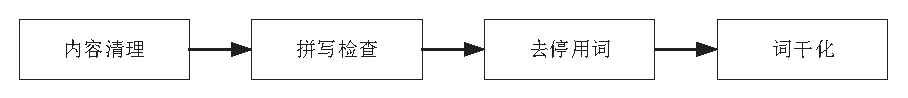
\includegraphics[width=\textwidth]{file_pre.eps}\\
  \caption{文本预处理过程}\label{fig:3-12}
\end{figure}
首先进行内容清理,即对文档中的句子进行清理,去掉数字、标点以及非字母符号,并将字母统一为小写。然后进行拼写检查,即对文档中的单词的拼写进行检查,将拼写错误的单词进行修正。然后我们去除句子中的停用词,例如``the"、``is"、``and"、``what"。最后,我们需要对英文单词进行词干化处理,主要包括将名词复数变为单数,将动词的过去时、进行时等时态变为最基本的形态。

\subsection{相似度计算}
在对Web服务的描述文档进行文本预处理后,每个Web服务的描述文档就可以看成一组词向量,即对Web服务$s$来说,它的描述文档就是$s = <word1,word2,word3...>$。

如图\ref{fig:12}我们对所有Web服务处理后的描述文档进行LDA主题模型训练, 可以最终得到两个分布,即文档-主题分布和主题-词频分布,此处我们主要用到文档主题分布,由于一个描述文档对应于一个Web服务,所以此处我们又称为服务-主题分布。
\begin{figure}[htbp]
  \centering
  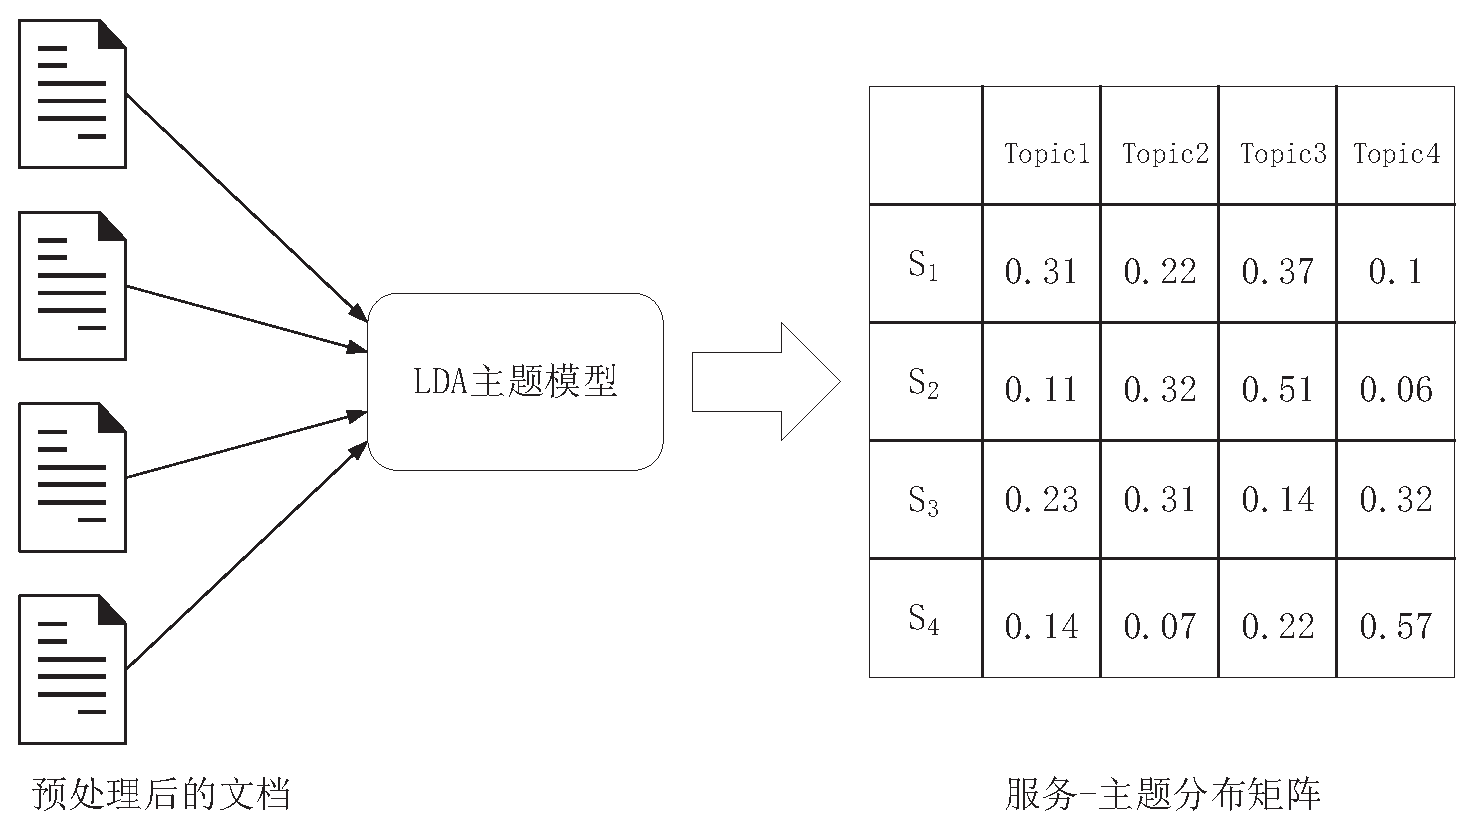
\includegraphics[width=0.8\textwidth]{LDAmatrix.eps}\\
  \caption{服务-主题分布生成示例图}\label{fig:12}
\end{figure}
根据服务-主题分布,对于Web服务$s_i$都可以用一个主题向量$d_i=<w_{i1},w_{i2},w_{i3}...w_{in}>$表示。$w_{ik}$表示服务$i$在主题$k$下的概率。本文采用余弦相似度来计算主题向量之间的相似性,主题相似度计算如下:
\begin{equation}
Sim_T(s_i,s_j)=\cos(\vec{d_i},\vec{d_j}) =\frac{\vec{d_i}\cdot \vec{d_j}}{\left \| \vec{d_i} \right \|\times \left \| \vec{d_j} \right \|}=\frac{\sum\limits_{k=1}^N w_{ik}w_{jk}}{\sqrt{\sum\limits_{k=1}^Nw_{ik}^{2}}\sqrt{\sum\limits_{k=1}^Nw_{jk}^{2}}}
\end{equation}
其中$Sim_T(s_i,s_j)$是服务$s_i$和服务$s_j$的主题相似度,$N$为主题的个数。

我们的主题相似度计算流程如图\ref{fig:3-13}所示。
\begin{figure}[htbp]
  \centering
  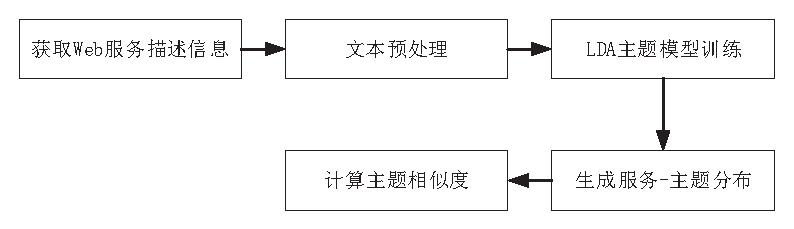
\includegraphics[width=\textwidth]{LDA_kuangjia.eps}\\
  \caption{主题相似度计算流程}\label{fig:3-13}
\end{figure}

\section{服务组合相似度}
当前的Web服务推荐中,Mashup应用所蕴含的服务组合信息没有引起足够的重视。什么是服务组合信息?我们以一个名为WunderWalk的Mashup应用为例,WunderWalk由两个Web服务API构成,分别是Google Maps和FourSquare。Mashup和API之间的组合关系即为服务组合信息。ProgrammableWeb网站的用户主要分为服务的开发者和服务的使用者,作为服务开发者,当我们对WunderWalk感兴趣的时候,我们是不是也有很大可能会对Google Maps以及Foursqure保持一定的兴趣呢?同样的,当我们对Google Maps感兴趣的时候,我们是不是也会对那些使用Google Maps构成的Mashup应用感兴趣呢?
下一节,我们将从两个角度探讨引入服务组合信息的意义。
\subsection{引入服务组合信息的意义}
我们认为,引入服务组合信息有以下两个优势:
\begin{enumerate}
\item \emph{Mashup中蕴含的服务组合关系,包含着服务之间的隐式联系}~以图\ref{fig:13}为例,
\begin{figure}[htbp]
  \centering
  
\includegraphics[width=0.5\textwidth]{Mashup-API.eps}\\
  \caption{Mashup-API调用关系图}\label{fig:13}
\end{figure}
$m_1$,$m_2$,$m_3$是三个Mashup,$a_1$,$a_2$,$a_3$,$a_4$是四个原子服务,其中$m_1$由$a_1$,$a_2$,$a_4$组合而成,那么当一个用户关注了$a_1$和$a_2$,将$a_4$推荐给该用户将是一个明智的选择。同样的,$m_1$也可以推荐给该用户,因为该用户关注的$a_1$和$a_2$是和$m_1$在组合关系上相关联的原子服务。当一个用户关注了Mashup应用$m_1$,那么该用户有很大可能也会对$m_3$感兴趣,因为$m_1$和$m_3$都调用一些公共的原子服务。我们对关注了WunderWalk的用户进行了统计,发现在关注WunderWalk的人当中,约有25\%的人也关注了Foursquare,有12.5\%的人关注了Google Maps,同时,在关注WunderWalk的人当中,约有20\%的人关注了一个叫EVMapper的Mashup应用,该Mashup由Google Maps和Eventful组合而成。


\item \emph{对主题信息的补充}~主题信息的引入,旨在能够为用户推荐那些功能上相似的服务,而引入服务组合信息,可以为推荐增加新的维度,帮助用户发现那些可能在功能上不相似但是具有服务组合关系的Web服务,比如,当一个用户关注了Foursquare,那么可以根据组合关系为用户推荐Google Maps,尽管这两个Web服务没有功能上的联系。
\end{enumerate}

\subsection{相似度计算}

为了能够量化服务组合关系,本文定义了服务组合相似度的。我们计算服务组合相似度主要分为两个部分:
\begin{enumerate}
\item \emph{根据Mashup的服务组合信息建立Mashup-API调用关系矩阵}~给定$M$个Mashup和$N$个API,我们可以建立一个$M \times N$的Mashup-API调用关系矩阵,矩阵中的元素由0和1构成,对于矩阵中第$i$行第$j$列的值若为1则表示Mashup $i$调用了API $j$,若为0则表示Mashup $i$没有调用API $j$。

\item \emph{根据调用关系矩阵计算Web服务之间的组合相似度}~在生成调用关系矩阵后,我们可以根据矩阵来计算Web服务之间的组合相似度。Web服务之间的组合相似度分为三种情况:(1)两个Web服务都是Mashup应用:我们假设这两个Mashup应用为Mashup $x$和Mashup $y$,那么这两个Mashup之间调用的公共API越多,则这两个Mashup越相似,如果两个Mashup之间没有公共调用的API,那么这两个Mashup组合相似度为0。如果两对Mashup调用的公共API个数相同,那么包含更多API的Mashup应该具有更低的相似度,为此我们定义两个Mashup之间的服务组合相似度$Sim_C(x,y)$如下:
\begin{equation}
Sim_C(x,y) = \frac{\left | A_1\bigcap A_2 \right |}{\left | A_1\bigcup A_2 \right |}\label{3-4}
\end{equation}
其中$A_1$,$A_2$为Mashup $x$和Mashup $y$所调用的API集合,公式\eqref{3-4}可以通过Mashup-API调用矩阵Mashup $x$和$y$的对应行求得。$Sim_C(x,y)$的值在0和1之间,值越大则表示越相似;(2)两个Web服务一个是Mashup一个是API:这种情况可以将该API看成是一个特殊的Mashup,该Mashup只调用一个API,那么此时这两个Web服务之间的组合相似度可以看成是两个Mashup之间的组合相似度,使用公式\eqref{3-4}来计算;(3)两个Web服务都是API:对于两个API $x$和$y$,我们着重看这两个API被哪些Mashup调用了,如果这两个API没有被任何Mashup同时调用,那么这两个API之间组合相似度为0,如果这两个API被很多Mashup同时调用,那么这两个API之间的组合联系就越强,即组合相似度就应该越大,同时,如果调用API $x$的Mashup数越多或者调用API $y$的Mashup数越多,则API $x$和API $y$之间的组合相关度应该被削弱,即组合相似度应该越低,因此,我们定义两个API之间的组合相似度$Sim_C(x,y)$如下:
\begin{equation}
Sim_C(x,y) = \left\{  
             \begin{array}{lr}  
             0, &\left | M_1\bigcup M_2 \right |=0\\  
             \frac{\left | M_1\bigcap M_2 \right |}{\left | M_1\bigcup M_2 \right |}, & \left | M_1\bigcup M_2 \right |\neq 0\\  
      
             \end{array}  
\right.
\end{equation}
其中,$M_1$是调用API $x$的Mashup集合,$M_2$是调用API $y$的Mashup集合,$\left | M_1\bigcup M_2 \right | =0$表示API $x$和API $y$没有被任何Mashup调用过。$Sim_C(x,y)$取值范围在0和1之间,值越大表示越相似。

\end{enumerate}

服务组合相似度的计算流程如图\ref{fig:3-14}所示。
\begin{figure}[htbp]
  \centering
  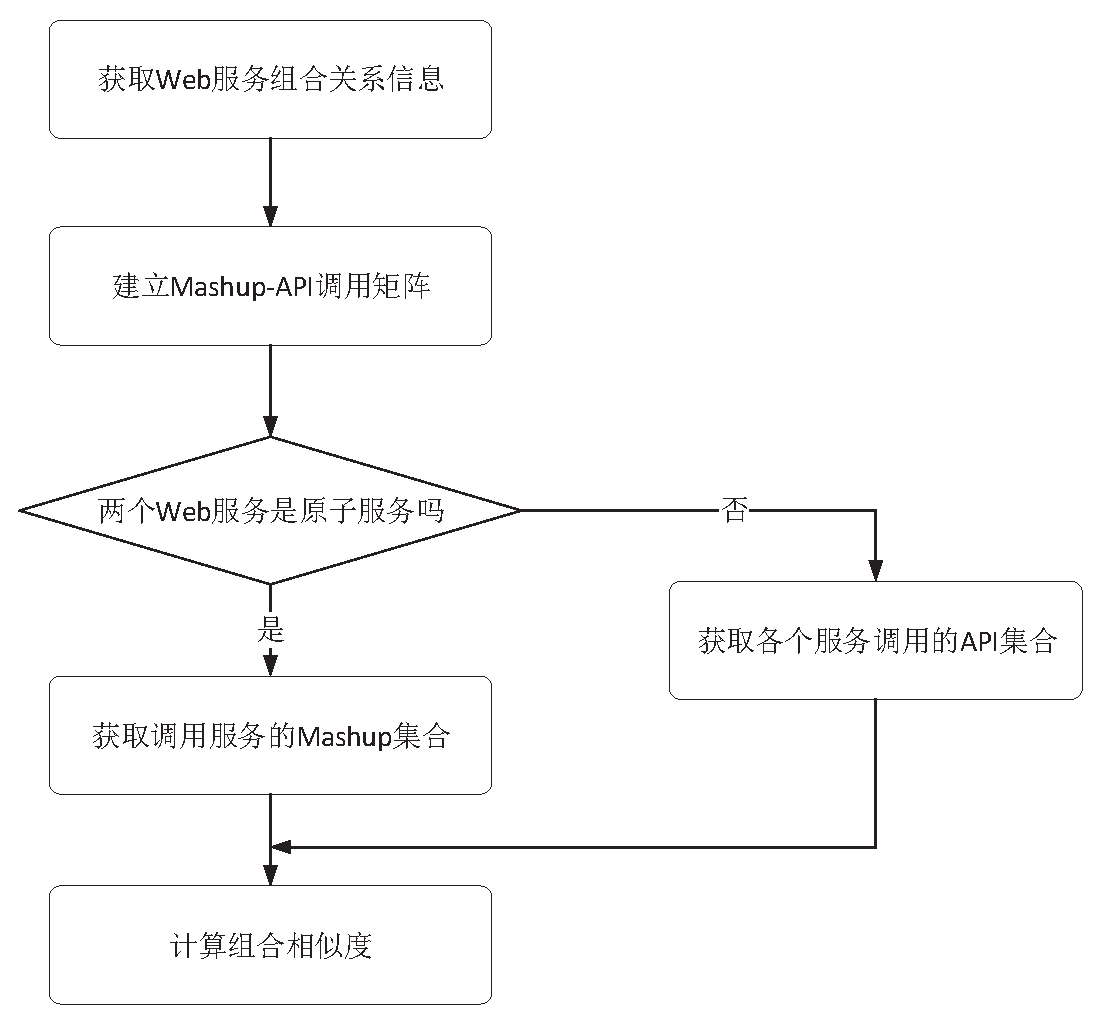
\includegraphics[width=0.8\textwidth]{Mashup_process.eps}\\
  \caption{服务组合相似度计算流程}\label{fig:3-14}
\end{figure}

\section{模型融合}
矩阵分解模型从用户历史偏好的数据集中训练出一个推荐模型,然后根据模型对用户的潜在偏好进行预测。矩阵分解模型不仅能带来很好的推荐结果,而且具有非常好的扩展性,能够融合各种特征,提升推荐的结果。

我们着重考虑的是带偏差的SVD分解模型。带偏差的SVD分解模型考虑用户和项目的偏差,即该模型认为,每个用户的评分都会有差异性,有的用户整体打分偏低,而有的用户打分会整体偏高。同样,每个项目的评分也是有偏差的。因此,带偏差的SVD分解建立的预测模型如下:
\begin{equation}
\hat{r}_{ui}=\mu +b_u+b_i+\bm{p_{u}}^T\bm{q_{i}}
\end{equation}
其中,$\hat{r}_{ui}$是用户评分的预测值,$\mu$表示训练集中所有用户的全局平均分,$b_u$是用户偏置项,表示了用户评分习惯的差异性,$b_i$是项目偏置项,表示了不同项目评分的差异性。$\bm{p_{u}} \in R^{f}$是用户$u$的潜在因子向量,$f$是潜在因子个数,$\bm{q_{i}} \in R^{f}$是项目$i$的潜在因子向量。

对于这样的预测模型,我们可以通过随机梯度下降的方法,求解以下目标函数来找到相应的参数的值:
\begin{equation}
\arg\min_{p_*,q_*,b_*}\sum \limits_{(u,i) \in T}(r_{ui}-\mu-b_u-b_i-p_u^Tq_i)^2+\lambda(\left \| p_u \right \|^2+\left \| q_i \right \|^2+b_u^2+b_i^2 )\label{3-8}
\end{equation}
其中,$r_{ui}$是训练集中的真实用户评分,$\lambda$是正则系数,用以防止过拟合,$p_*$,$q_*$,$b_*$表示要求解的所有用户潜在因子向量,项目潜在因子向量以及偏差。

在前面的小节中,我们计算得到了Web服务之间的主题相似度$Sim_T$和服务组合相似度$Sim_C$,根据主题相似度,我们定义服务$i$的在主题层面上的邻居集合$N^k_t(i)$如下:
\begin{equation}
N^k_t(i)=\left \{ l|l\in Top^k(i),Sim_T(i,l)>0,i\neq l \right \}
\end{equation}
其中,$Top^k(i)$表示与服务$i$在主题相似度上最相近的$k$个Web服务的集合,$Sim_T(i,l)$是服务$i$和服务$l$的主题相似度。

同样的,我们定义Web服务$i$在服务组合层面上的邻居集合$N^k_c(i)$如下:
\begin{equation}
N^k_c(i)=\left \{ l|l\in Top^k(i),Sim_C(i,l)>0,i\neq l \right \}
\end{equation}
其中,$Top^k(i)$表示与服务$i$在服务组合相似度上最相近的$k$个Web服务的集合,$Sim_C(i,l)$是服务$i$和服务$l$的服务组合相似度。

我们将主题信息和服务组合信息融入到SVD分解模型中,通过两个权重参数来调整主题信息、服务组合信息所占的比重,因此构造如下评分预测:
\begin{equation}
\hat{r}_{us} = \mu+b_u+b_s+(1-\alpha-\beta)p_u^T\cdot q_s+\alpha \sum \limits_{l \in N^{k_1}_t(s)} \omega_{sl}p_u^T\cdot q_l+\beta \sum \limits_{k \in N^{k_2}_c(s)} \eta_{sk}p_u^T\cdot q_k\label{3-12}
\end{equation}

其中,$\hat{r}_{us}$是用户$u$对服务$s$的评分的估计值,$\alpha$是主题信息的平衡系数,$\beta$是服务组合信息的平衡系数,$N^{k_1}_t(s)$是与服务$s$在主题相似度上最相近的$k_1$个服务的集合,$N^{k_2}_c(s)$是与服务$s$在服务组合相似度上最相近的$k_2$个服务的集合,$\omega_{sl}$是服务$s$和服务$l$的主题相似性权重,计算如下:
\begin{equation}
\omega_{sl} = \frac{Sim_T(s,l)}{\sum \limits_{i \in N^{k_1}_t(s)}Sim_T(s,i)}
\end{equation}
同样的,$\eta_{sk}$是服务$s$和服务$k$的服务组合相似性权重,计算如下:
\begin{equation}
\eta_{sk} = \frac{Sim_C(s,k)}{\sum \limits_{i \in N^{k_2}_c(s)}Sim_C(s,i)}
\end{equation}

该预测模型可以通过如下的目标函数求解:
\begin{equation}
\arg\min_{p_*,q_*,b_*}\sum \limits_{(u,s) \in T}(r_{us}-\hat{r}_{us})^2+\lambda(\left \| p_u \right \|^2+\left \| q_s \right \|^2+\sum \limits_{l \in N^{k_1}_t(s)}\left \| q_l \right \|^2+\sum \limits_{k \in N^{k_2}_c(s)}\left \| q_k \right \|^2+b_u^2+b_s^2 )
\end{equation}

我们可以通过随机梯度下降的方式求解该目标函数,随机梯度下降的更新公式如下:
\begin{equation}
\begin{split} 
& b_u\leftarrow  b_u+\gamma\cdot (e_{us}-\lambda b_u)\\
& b_s\leftarrow  b_s+\gamma\cdot (e_{us}-\lambda b_s)\\
& p_u\leftarrow  p_u+\gamma\cdot (e_{us}((1-\alpha-\beta)q_s+\alpha \sum \limits_{l \in N^{k1}_t(s)} \omega_{sl}q_l+\beta \sum \limits_{k \in N^{k2}_c(s)} \eta_{sk}q_k)-\lambda \cdot p_u)\\
& q_s\leftarrow  q_s+\gamma\cdot ((1-\alpha-\beta)e_{us}\cdot p_u-\lambda \cdot q_s)\\
& \forall l \in N^{k_1}_t(s):\\
& q_l\leftarrow  q_l+\gamma\cdot (e_{us}\cdot \alpha\cdot \omega_{sl}\cdot p_u-\lambda \cdot q_l)\\
& \forall k \in N^{k_2}_c(s):\\
& q_k\leftarrow  q_k+\gamma\cdot (e_{us}\cdot \beta\cdot \eta_{sk}\cdot p_u-\lambda \cdot q_k)
\end{split}
\end{equation}
其中,$e_{us} = r_{us}-\hat{r}_{us}$,$\gamma$是学习率,用以控制随机梯度下降的速度。

我们的融合了主题信息和服务组合信息的SVD分解算法(TC-SVD)如下:

\begin{algorithm2e}
	\caption{融合主题信息与服务组合信息的SVD分解模型}
	\label{labelpropagation}
	\KwIn{watchlist set $W$, description set $D$, compositional information set $H$, $F$, $K_1$, $K_2$, $\lambda$, $\gamma$, $M$, $N$}
	\KwOut{Model parameters $B_U,B_S,P_{M\times F}, Q_{N \times F}$}
\SetKwFunction{GetRatingsByWatchlist}{GetRatingsByWatchlist}
\SetKwFunction{GetTopicSimilarity}{GetTopicSimilarity}
\SetKwFunction{GetCompositionalSimilarity}{GetCompositionalSimilarity}
\SetKwFunction{GetRatingsByWatchlist}{GetRatingsByWatchlist}
\SetKwFunction{GetTopicNeighborSet}{GetTopicNeighborSet}
\SetKwFunction{GetCompositionalNeighborSet}{GetCompositionalNeighborSet}
\SetKwFunction{GenerateModelParameters}{GenerateModelParameters}
\textbf{\emph{/*===== Ratings Calculation =====*/}}\\
rating matrix $R_{M \times N} \gets \GetRatingsByWatchlist{$W$}$\;
\textbf{\emph{/*===== Similarity Calculation =====*/}}\\
topic similarity $T_{N \times N} \gets \GetTopicSimilarity{$D$}$\;
compositional similariy $C_{N \times N} \gets \GetCompositionalSimilarity{$T$}$\;

\textbf{\emph{/*===== Model learning =====*/}}\\
$B_U,B_S  \gets ( 0,0,\cdots,0)$\;
$P_{M\times F},Q_{N \times F}\sim \mathcal N(0,0.005)$\;
%\STATE  Compute the Topic Neighbour set $N^{k1}_t$ of service 
$N^{k_1}_t \gets \GetTopicNeighborSet{$T$}$\;
%\STATE  Compute the Compositional Neighbout set $N^{k2}_c$ of service
$N^{k_2}_c \gets \GetCompositionalNeighborSet{$C$}$\;
\While{the stop criterion is met}{
	\For{$(u,s,r) \in R$}{
		$e_{us} \gets r_{us}-\hat{r}_{us}$\;
		update $B_U(u),B_S(s),P(u),Q(s)$ by $\eqref{3-16}$\;
	}
	$\gamma \gets 0.99*\gamma$\;
}
\GenerateModelParameters{}\;
\end{algorithm2e}

\section{算法实现}
本章算法的实现主要是基于Gang Tian等人\cite{Tian2014Time}提供的数据集pweb\footnote{http://tiangang.theclever.me/supplements.html/},该数据集爬取了ProgrammableWeb网站截止2013年11月25日的相关数据,包括10000多个Web服务,7000多个Mashup以及280000多条用户watchlist记录。我们算法主要包括评分计算、主题相似度计算、组合相似度计算和模型融合等几个模块,我们基于Python 2.7以及Python第三方库实现了各个模块,核心模块的总代码量约为1300多行。图\ref{fig:23}是我们的算法代码模块图,下面将对模块中主要函数的功能作简要介绍。
\begin{figure}[htbp]
  \centering
  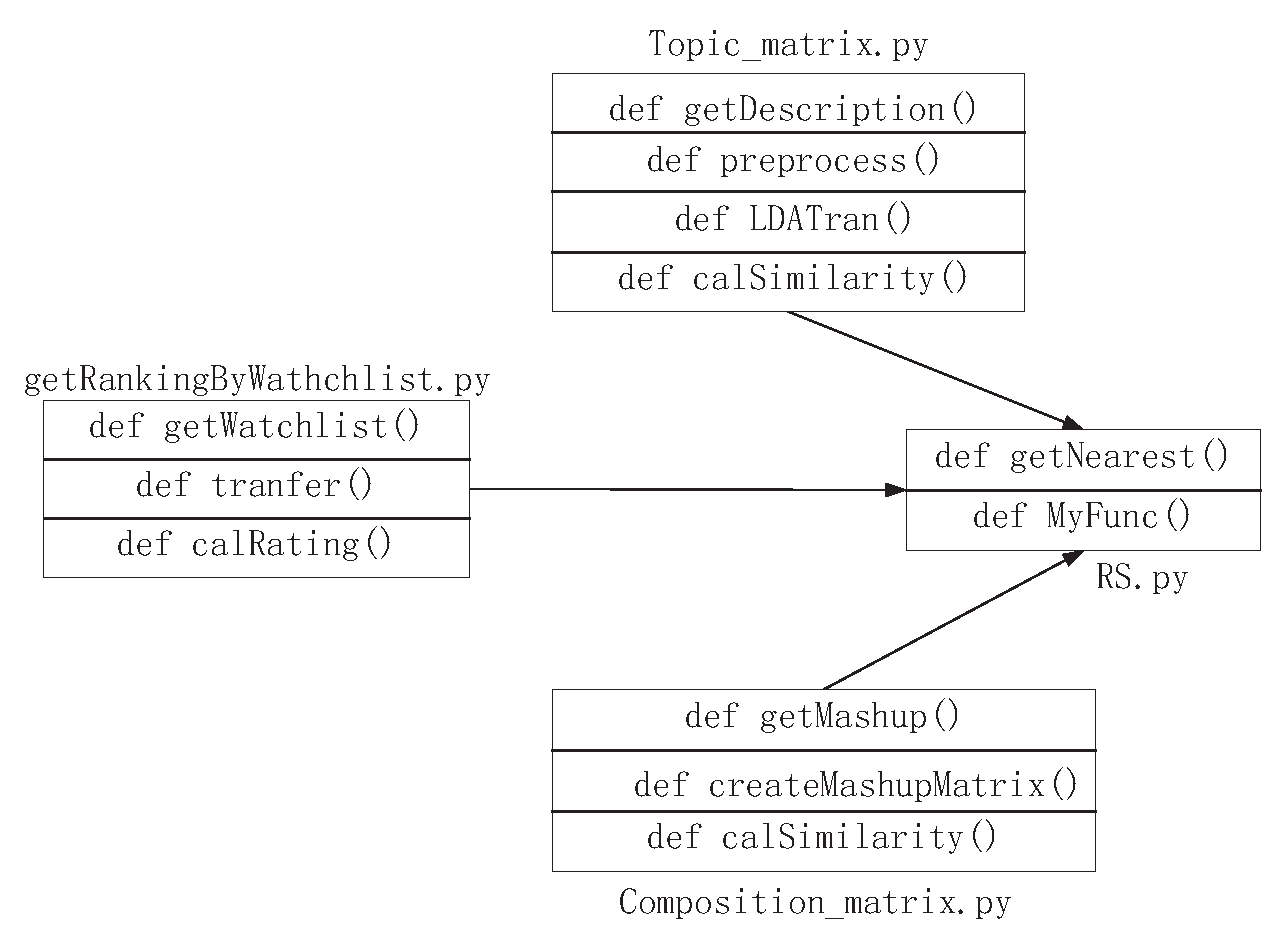
\includegraphics[width=\textwidth]{Code1.eps}\\
  \caption{算法代码模块图}\label{fig:23}
\end{figure}
\begin{enumerate}
\item \emph{评分计算}~我们在getRankingByWatchlist.py中实现了评分计算,该模块主要有三部分,函数getWatchlist负责从pweb数据库中提取用户的观察列表信息,形式为$<user,url,id,date>$,分别对应了用户、服务地址、数据库主键id以及时间。接下来我们通过函数tranfer来对$url$和$date$进行处理,从$url$中提取服务名,将$date$由字符串类型转换为日期类型,转换后我们得到一组$<user,service,time>$。最后,我们统计各服务在用户列表中出现的频次,根据\eqref{eq:3-1}计算评分,生成一组$<user,service,rating,time>$。
\item \emph{主题相似度计算}~我们在Topic\li matrix.py中实现了主题相似度的计算,首先通过函数getDescription从pweb数据库提取服务的描述文档,然后函数prepross对文档进行预处理,接着将预处理后的文档通过函数LDATran进行LDA主题模型的训练,最后函数calSimilarity利用生成的文档-主题分布计算余弦相似度,得到主题相似度矩阵。

\item \emph{组合相似度计算}~由于在pweb数据集中没有服务组合关系,我们利用爬虫工具爬取了ProgrammableWeb网站上的全部Mashup和API的组合信息,存在Composition\li Mashup.xlsx中。我们利用函数getMashup从数据库中提取Mashup并利用爬取的信息来找到Mashup的调用关系,利用函数createMashupMatrix建立Mashup和API的调用关系矩阵。函数calSimilarity根据调用关系矩阵,计算组合相似度。

\item \emph{模型融合}~我们在RS.py中实现了模型的融合和训练,该模块主要有两个部分,函数getNearest主要是根据相似度矩阵寻找每个Web服务的最近邻,函数MyFunc主要是将主题信息和组合信息融合并利用随机梯度下降的方法进行训练,产生预测。另外,本模块还实现了数据加载,数据集划分,评估指标计算以及大量的协同过滤算法用以对比验证。
\end{enumerate}

\section{实验设计}
\subsection{实验数据及评估指标}
为了评估主题信息和服务组合信息对服务推荐的影响,我们选择了观察列表中至少包含50个服务的用户,一共有510个用户和4813个服务被选中,其中共有2713个原子Web服务和2100个Mashup,如表\ref{table:3-6}所示。
\begin{table}[h]
\centering
\caption{ProgrammableWeb数据集数据统计}
\label{table:3-6}
\begin{tabular}{|c|c|}
\hline
用户数            & 510     \\ \hline
原子Web服务数       & 2713    \\ \hline
Mashup数        & 2100    \\ \hline
Mashup包含的平均服务数 & 2.2     \\ \hline
数据稀疏率          & 99.13\% \\ \hline
\end{tabular}%
\end{table}
本实验主要使用的是评分预测模型,因此我们采用的评估指标是RMSE和MAE。


\subsection{准确性验证}
为了评测本章提出的服务推荐算法TC-SVD的性能,我们将它与5个典型的推荐方法进行了比较,这几个算法简介如下:

UPCC:一种典型的基于用户的算法,使用皮尔逊相关系数作为相似度\cite{Breese1998Empirical}。

IPCC:一种基于项目的协同过滤算法,使用皮尔逊相关系数度量项目间的相似度\cite{Kang2012AWSR}。

RSVD:引入了正则项以防止过拟合的SVD分解方法。

RBSVD:引入了偏置项和正则项的SVD分解方法\cite{Koren2010Collaborative}。

TASR:引入了时间维度的矩阵分解方法\cite{Tian2014Time}。

TC-SVD:我们的方法。
我们将数据集划分为训练集和测试集,训练集和测试集的比例介于0.5到0.9之间,从而形成了不同稀疏率(data sparsity)的训练矩阵,表\ref{table:3-8}是不同稀疏率下各算法的性能。

\begin{table}[h]
\centering
\caption{各算法RMSE/MAE比较}
\label{table:3-8}
\resizebox{\textwidth}{!}{%
\begin{tabular}{|c|c|c|c|c|c|c|c|c|c|c|}
\hline
\multirow{5}{*}{Algorithm} & \multicolumn{10}{c|}{Training Set Ratio}                                                                                                                                             \\ \cline{2-11} 
                           & \multicolumn{2}{c|}{0.9}           & \multicolumn{2}{c|}{0.8}           & \multicolumn{2}{c|}{0.7}          & \multicolumn{2}{c|}{0.6}           & \multicolumn{2}{c|}{0.5}          \\ \cline{2-11} 
                           & \multicolumn{10}{c|}{Data Sparsity}                                                                                                                                                  \\ \cline{2-11} 
                           & \multicolumn{2}{c|}{0.9924}        & \multicolumn{2}{c|}{0.9933}        & \multicolumn{2}{c|}{0.9941}       & \multicolumn{2}{c|}{0.9950}        & \multicolumn{2}{c|}{0.9958}       \\ \cline{2-11} 
                           & RMSE            & MAE              & RMSE            & MAE              & RMSE            & MAE             & RMSE            & MAE              & RMSE           & MAE              \\ \hline
UPCC                       & 0.0272          & 0.0196           & 0.0277          & 0.0198           & 0.0278          & 0.0202          & 0.0287          & 0.0210           & 0.0295         & 0.0215           \\ \hline
IPCC                       & 0.0302          & 0.0219           & 0.0301          & 0.022            & 0.0302          & 0.0221          & 0.0306          & 0.0225           & 0.0310         & 0.0228           \\ \hline
RSVD                       & 0.0155          & 0.00836          & 0.0171          & 0.00864          & 0.0174          & 0.00923         & 0.0184          & 0.0101           & 0.0203         & 0.0113           \\ \hline
RBSVD                      & 0.0128          & 0.00678          & 0.0129          & 0.00678          & 0.0132          & 0.00680         & 0.0145          & 0.00732          & 0.0145         & 0.00757          \\ \hline
TASR                       & 0.0125          & 0.00672          & 0.0128          & 0.00688          & 0.0129          & 0.0694          & 0.0143          & 0.00756          & 0.0141         & 0.0077           \\ \hline
\textbf{TC-SVD}            & \textbf{0.0124} & \textbf{0.00633} & \textbf{0.0127} & \textbf{0.00639} & \textbf{0.0130} & \textbf{0.0647} & \textbf{0.0142} & \textbf{0.00713} & \textbf{0.0140} & \textbf{0.00738} \\ \hline
\end{tabular}%
}
\end{table}
由表\ref{table:3-8}可知,在不同稀疏率下,基于模型的方法普遍比基于邻域的方法具有更好的准确度,和带偏差的SVD分解方法相比,我们的方法引入了主题信息和服务组合信息, 在不同稀疏率下都具有更低的RMSE和MAE,和考虑时序的模型TASR相比,我们的方法在不同稀疏率下MAE的值都要更低,而RMSE的值只在稀疏率为0.7的时候表现不佳,在其他的稀疏率下都要略优于时序模型。总体而言,我们的方法在训练集比重占0.9时,相对不引入主题信息和服务组合信息的RBSVD方法,在RMSE上提升了3.2\%,在MAE上提升了7.1\%。相对于引入了时序的TASR模型,RMSE提升了0.8\%,在MAE上提升了5.8\%。这说明,将主题信息和服务组合信息融入到服务推荐的过程中,可以有效地提高推荐的预测性能。


\subsection{各参数影响分析}
我们的方法中的参数主要有平衡因子$\alpha$,$\beta$,主题邻居数$K_1$和组合邻居数$K_2$以及潜在因子个数$F$。实验中,我们为了简化调参的过程,设定主题邻居数$K_1$和组合邻居数$K_2$相同,即$K_1=K_2$,
我们将正则项系数$\lambda$设为0.001。下面将对各参数的影响作出分析。
\begin{arabicenum}
\item 平衡因子$\alpha$,$\beta$

实验中我们通过两个平衡因子$\alpha$和$\beta$来控制主题信息和服务组合信息的权重。图\ref{lab-1},\ref{lab-2}是$\alpha$对RMSE和MAE的影响,$\alpha$控制着主题信息的权重,我们设置邻居个数为15,主题个数为50,潜在因子个数为30,$\beta$数值为0.2,取$\alpha$的值在$[0,0.5]$之间。我们发现,随着$\alpha$的增大,RMSE和MAE的值在逐渐减小,准确性在上升,当$\alpha=0.1$时,RMSE达到最小,当$\alpha=0.2$时,MAE达到最小,随后当$\alpha$增大,RMSE和MAE的值都在增大,这说明准确性在下降,这可能是由于主题信息的加入影响到了其他信息所占的比重。
\begin{figure}[h]
\centering
\begin{minipage}[t]{0.48\textwidth}
\centering
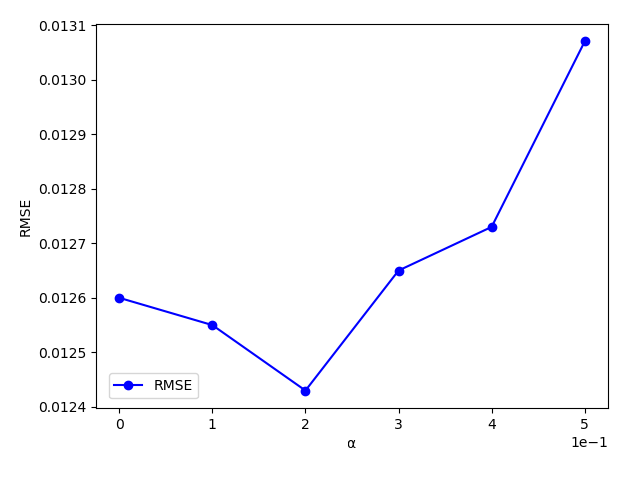
\includegraphics[width=7cm]{alpha_a.png}
\caption{$\alpha$对RMSE的影响}\label{lab-1}
\end{minipage}
\begin{minipage}[t]{0.48\textwidth}
\centering
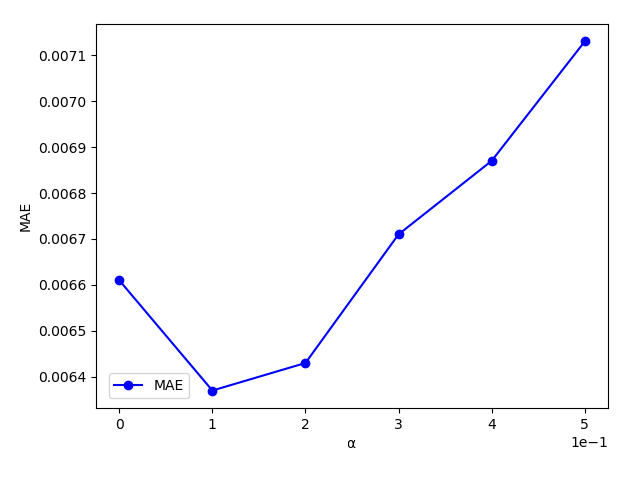
\includegraphics[width=7cm]{alpha_b.png}
\caption{$\alpha$对MAE的影响}\label{lab-2}
\end{minipage}
\end{figure}

\begin{figure}[htbp]
\centering
\begin{minipage}[t]{0.48\textwidth}
\centering
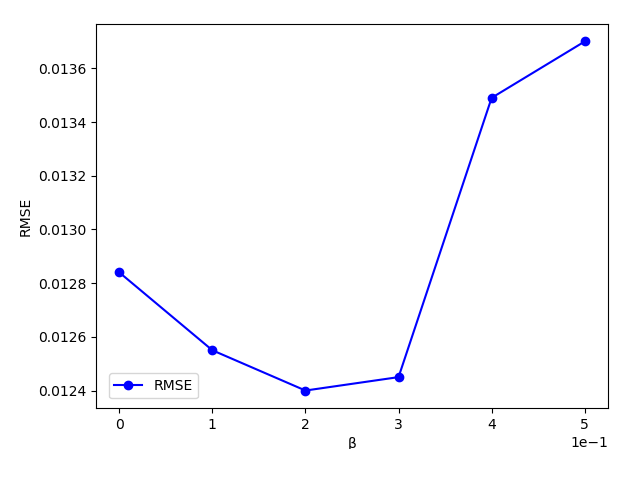
\includegraphics[width=7cm]{beta_a.png}
\caption{$\beta$对RMSE的影响}\label{lab-3}
\end{minipage}
\begin{minipage}[t]{0.48\textwidth}
\centering
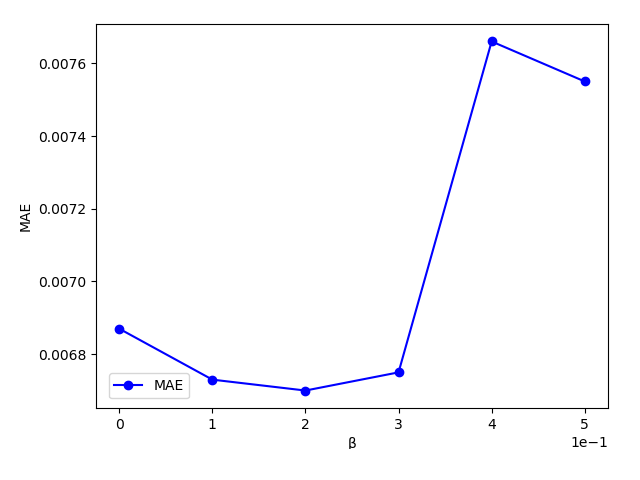
\includegraphics[width=7cm]{beta_b.png}
\caption{$\beta$对MAE的影响}\label{lab-4}
\end{minipage}
\end{figure}

图\ref{lab-3},\ref{lab-4}是$\beta$对RMSE和MAE的影响,从图中可以看出,随着$\beta$的增大,RMSE和MAE都在下降,准确性在提高,当$\beta=0.2$时,RMSE和MAE都取得最小值,后面随着$\beta$的值的不断上升,RMSE和MAE的值也在上升,这说明推荐的准确性在下降,这是由于随着服务组合关系的影响权重在增大,影响了其他信息的所占的权重,从而带来了不好的效果。$\beta=0.2$使得RMSE和MAE取得最小值,也说明了将服务组合信息融入推荐确实能够提升推荐的准确性。

\item 主题/服务组合邻居数$K_1$

实验中我们让主题邻居以及组合邻居的个数相同,我们将邻居个数$K_1$在区间[5,50]中调整,结果如图\ref{lab-5},\ref{lab-6}所示,随着邻居数的增加,RMSE和MAE的值都在降低,当$K_1$在15到50之间增长时,RMSE和MAE的值在上下波动,这可能是由于我们默认将主题信息邻居个数和服务组合邻居个数设置为相同,而邻居数在15到50之间时,这两种信息会对预测结果互相干扰。
\begin{figure}[htbp]
\centering
\begin{minipage}[t]{0.48\textwidth}
\centering
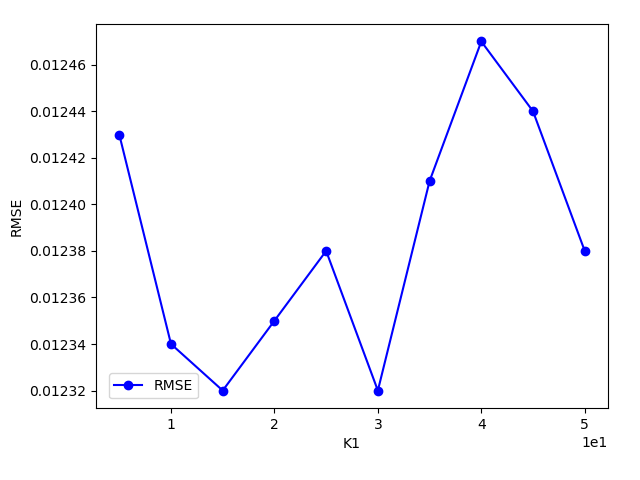
\includegraphics[width=7cm]{neighbour_a.png}
\caption{$K1$对RMSE的影响}\label{lab-5}
\end{minipage}
\begin{minipage}[t]{0.48\textwidth}
\centering
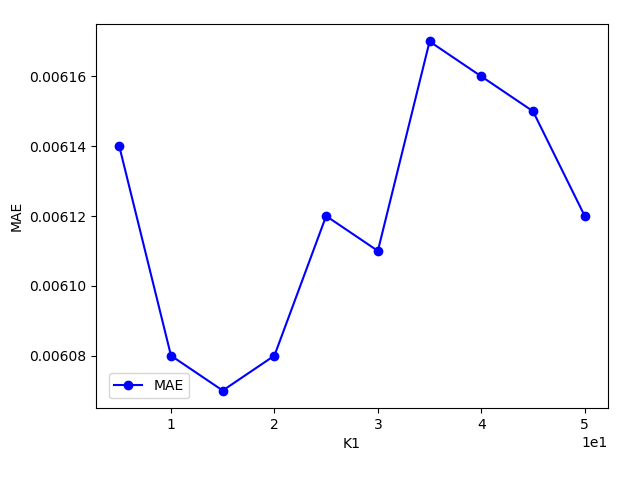
\includegraphics[width=7cm]{neighbour_b.png}
\caption{$K1$对MAE的影响}\label{lab-6}
\end{minipage}
\end{figure}

\begin{figure}[htbp]
\centering
\begin{minipage}[t]{0.48\textwidth}
\centering
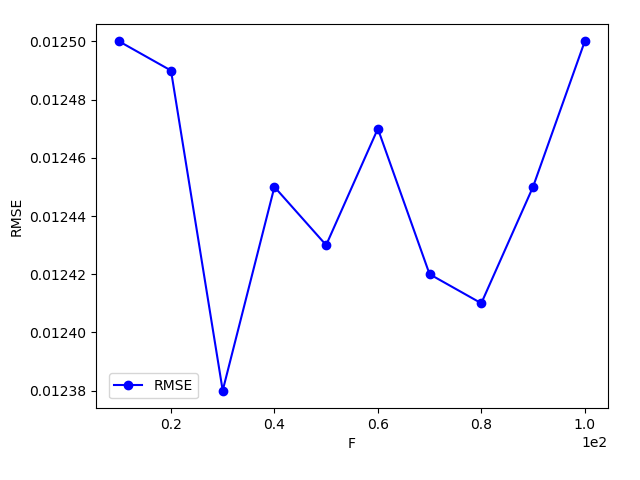
\includegraphics[width=7cm]{F_a.png}
\caption{$F$对RMSE的影响}\label{lab-7}
\end{minipage}
\begin{minipage}[t]{0.48\textwidth}
\centering
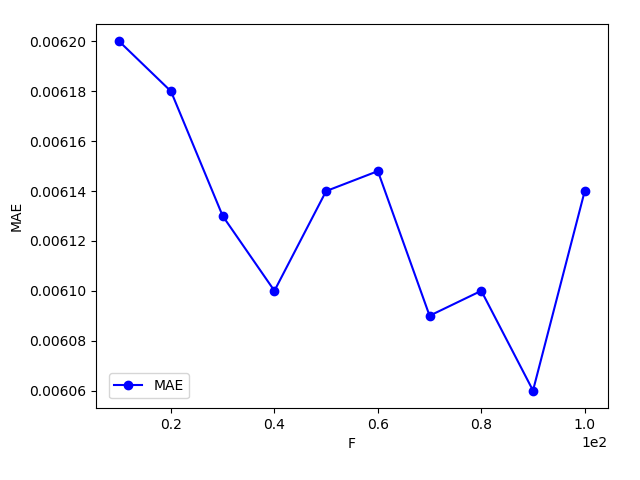
\includegraphics[width=7cm]{F_b.png}
\caption{$F$对MAE的影响}\label{lab-8}
\end{minipage}
\end{figure}

\item 潜在因子个数$F$

我们设置邻居数为15,$\alpha=0.2$,$\beta=0.2$,主题个数为50,将潜在因子个数$F$在区间[10,100]中递增,结果如图\ref{lab-7},\ref{lab-8}所示,我们发现,随着潜在因子个数的增加,RMSE和MAE都在减小,在$F=30$时,RMSE达到最小值,随后RMSE在上下波动,并在$F=80$以后开始增大,可能是由于随着$F$的增大,潜在因子维度不断增大,训练导致的数据过拟合现象开始越来越明显。同样的,当$F=90$时,MAE取得最小值,随后也开始增大。我们为了减小计算开销,实验中最终设定的潜在因子个数为30。

\end{arabicenum}
\section{本章小结}

在这一章,我们提出了一种融合了主题信息和服务组合信息的Web服务推荐算法,我们首先介绍了研究这一问题的背景,以及我们的主要研究对象ProgrammableWeb网站,然后介绍了引入主题信息和服务组合信息的动机和意义,并给出了主题相似度和服务组合相似度的计算方法,最后我们将主题信息和服务组合信息融合进SVD分解模型,并基于ProgrammableWeb网站的真实数据集来验证了我们的方法的有效性。
%%%%%%%%%%%%%%%%%%%%%%%%%%%%%%%%%%%%%%%%%%%%%%%%%%%%%%%%%%%%%%%%%%%%%%%%%%%%%%%
\chapter{基于重排名的服务推荐多样性提高算法}\label{chapter_scalefree}
\section{问题背景}
目前,大多数Web服务推荐的研究都是基于精度、召回、均方根误差等准确性指标,这些推荐算法力求通过在准确性指标上的提升来更好地预测用户的潜在兴趣,为用户推荐满意的服务。然而, 文献\cite{Cremonesi2011Looking}表明,推荐的高精度不一定意味着较高的用户满意度。一方面,推荐列表中推荐的项目通常与用户的历史行为有着一定的关联性,而用户通常希望推荐列表中除了那些他们认为理所当然的推荐项目外,还需要有一点点惊喜。另一方面,通常具有高精度的推荐算法倾向于向用户推荐流行的项目,对于那些被少部分用户喜欢的,较为冷门的项目则难以被推荐。这会导致推荐系统中的项目,热门的项目更加热门,冷门的项目更加冷门。我们统计了ProgrammableWeb数据集中的每个服务的用户关注数,我们发现关注数最多的20\%的服务,获得了大约67.9\%的用户评分,而关注数最多的100个服务,获得了大约32.5\%的用户评分。这表明,ProgrammableWeb网站上已经出现了大量的长尾服务\cite{Anderson2006The,Levy2010Music},因此我们在基于ProgrammableWeb网站作服务推荐时,考虑推荐的多样性是很有必要的。

在服务推荐中考虑推荐的多样性,有以下好处:对Web服务而言,冷门的服务有了更多被推荐给用户的机会,可以避免热门的服务越来越热门,冷门的服务无人问津的情况。对ProgrammableWeb网站的用户而言,可以帮助用户发现他们潜在喜欢的服务,也能发现一些用户意想不到的服务,给用户带来惊喜。同时,用户接触到更多样的服务,也能拓展用户的视野\cite{Cheng2017Learning}。对ProgrammableWeb网站而言,可以让网站的大多数服务都有机会被用户发现, 而不是只集中在少部分热门服务,更有利于网站的运营,增加网站的商业价值。

文献\cite{Zhou2010Solving}指出,提高推荐系统的多样性通常会降低系统的准确性,这也符合我们的直觉,即冷门的物品往往只被少数人所喜欢,如果把冷门的物品推荐给不喜欢它的用户,显然会造成准确性的下降。推荐的多样性问题研究的难点,就是如何在准确性和多样性之间找到一个平衡,使得推荐结果可以在尽可能少的损失准确性的同时,尽可能多的提升推荐的多样性。

本章主要基于重排名模型,提出了一种考虑用户偏差的改进重排名算法,可以在尽可能少地牺牲准确性的情况下,尽可能多地提高推荐的多样性。

\section{用户评分计算}

在ProgrammableWeb网站中,用户的显式评分信息往往很难获取,很多用户往往也不会给喜欢的服务打一个显式评分,因此在上一章中,我们利用用户观察列表中的隐式反馈信息来计算用户评分,这种方法计算的评分在[0,1]之间。本章我们希望得到一个5分制的评分集合,因此考虑对上一章的评分计算方式加以改进。图\ref{fig:4-1}是我们评分计算模块的基本框架。总共分为三个部分,即平均评分矩阵,时间权重矩阵和频率权重矩阵。下面我们将对这三个部分进行介绍。
\begin{figure}[htbp]
  \centering
  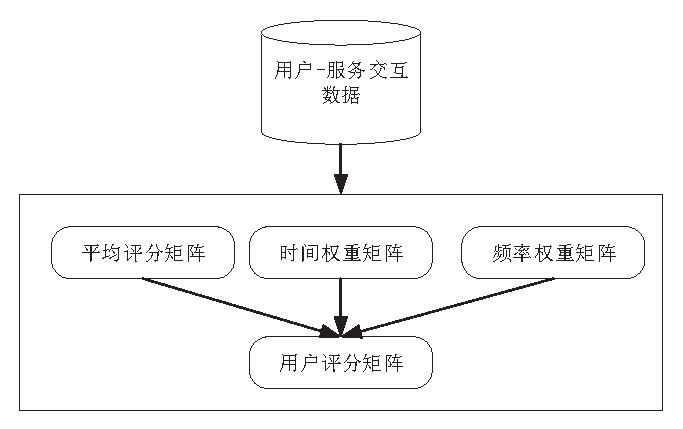
\includegraphics[width=0.8\textwidth]{rating.eps}\\
  \caption{用户评分计算框架}\label{fig:4-1}
\end{figure}

ProgrammableWeb网站中每个Web服务都有一个显式评分,即该服务的用户给出的显式评分反馈的平均值。这样的平均评分反应了用户对这种Web服务的整体评价。通过这些平均评分,我们可以建立平均评分矩阵$A \in R^{m \times n}$,其中$m$表示用户的数量,$n$表示服务的数量。平均评分矩阵$A$中的项$a_{ij}$定义如下:
\begin{equation}
a_{ij}= \begin{cases}r_{j} & if \ s_j \in Watchlist_i\\0 & otherwise \end{cases}
\end{equation}
其中,$r_j$表示服务$s_j$的平均评分,$r_j \in \left [0,5 \right ]$,$Watchlist_i$表示用户$i$的观察列表。

通常用户对服务的兴趣会随着时间的推移而逐渐减弱,同时我们也认为在提高多样性的过程中,那些较为新的服务相对于旧的服务应该具有更高的推荐优先级,因此我们在评分计算的过程中,考虑了时间权重矩阵。我们采用和文献\cite{Zhang2014Web}相同的方式对时间进行建模,即认为用户的兴趣随时间衰减的过程类似于物体冷却的过程,随着时间增长,一个热的物体的温度会逐渐降低直至等于室温,因此我们时间权重矩阵中的项$b_{ij}$定义如下:
\begin{equation}
b_{ij}= \begin{cases} \exp(-\alpha \times order(i,j))& if \ s_j \in Watchlist_i\\0 & otherwise \end{cases}\label{eq:4-1}
\end{equation}
其中$\alpha$用来控制用户兴趣随时间的衰减速度,本文设置为0.5,$order(i,j)$表示服务$s_j$在用户$i$中的观察列表中按照时间顺序出现的次序,若是最新的,则设置为0。$b_{ij}$的取值在[0,1]之间,越接近1表示该服务出现在用户观察列表的时间越近,越接近0则表示该服务相对用户越旧。

频率权重矩阵$C \in R^{m \times n}$即上一章计算的用户评分矩阵,通过用户观察列表中服务的更新频率与服务的受欢迎程度之间的隐式反馈信息计算的用户评分,该评分取值在$\left [0,1 \right ]$之间,Web服务的更新频率越高,关注的人数越多,该服务的评分越高。

我们综合了平均评分矩阵、时间权重矩阵和频率权重矩阵,得到我们最终的用户评分矩阵$R_{m \times n}$如下:
\begin{equation}
R_{m \times n} = (\lambda B_{m \times n}+(1-\lambda) C_{m \times n})\cdot A_{m \times n}\label{eq:4-2}
\end{equation}
其中$\lambda$是用来控制两个权重矩阵的比重,本文取0.5,$\cdot$是矩阵点乘,表示两个相同维度的矩阵对应位置相乘。

通过对ProgrammableWeb网站的用户交互数据进行提取,我们建立了混合评分矩阵,量化了用户偏好,该矩阵取值在[0,5]之间,方便我们对推荐的多样性进行进一步研究。

\section{考虑用户偏差的重排名算法}
经典的重排名算法使用固定阈值来调节推荐列表的准确性和多样性,但是用户是有差异的,使用统一的阈值来过滤用户评分,会影响模型的准确度,因此本章提出了考虑用户偏差的重排名算法。
\subsection{用户偏差}
在引入用户偏差之前,我们先给出服务流行度的定义,对于服务$i$,流行度定义$p_i$如下:
\begin{equation}
p_i = \left | \left \{ u \in U|\exists r_{ui}\right \} \right |
\end{equation}
其中$U$为用户集合,$r_{ui}$为用户$u$对服务$i$的评分。

服务流行度表示喜欢该Web服务的用户数量。对于一个Web服务,如果喜欢该服务的用户越多,则该服务越热门,而喜欢该服务的用户越少,则该服务越冷门。一般而言,推荐冷门的物品会使系统的准确性降低,但是此时系统的多样性会增加,此时用户反而容易发现一些新颖的未接触过的物品\cite{钟足峰2017可提高多样性的基于重排序图书推荐算法研究}。

对于用户偏差,我们认为主要体现在以下两个方面:

\begin{enumerate}
\item \emph{用户评分的差异性}~不同的用户评分习惯不同,有的用户评分比较严格,评分整体偏低,而有的用户则比较宽松,评分整体偏高。例如,在一个5分制的推荐系统中,用户$A$打分很严格,对喜欢的物品也只打3分,那么当评分阈值大于3分时,重排名将会对该用户失去作用,而用户$B$打分很宽松,对不喜欢的物品也打3分,那么当评分阈值小于3时,用户$B$将完全按照流行度进行排名。所以使用重排名算法时,考虑用户评分的差异性很有必要。

\item \emph{用户兴趣分布的差异性}~不同的用户兴趣分布不同,有的用户喜欢的都是偏热门的服务,那么给这样的用户推荐很多冷门的服务就不是太合适,相反的,有的用户兴趣分布较广,喜欢的服务中既有热门的又有冷门的服务,那么为这样的用户适当冷门服务就理所应当。因此,考虑用户兴趣分布的差异性也是有必要的。
\end{enumerate}

因此,在进行重排序的时候,相对于固定阈值的重排名模型,充分考虑用户的评分差异性和用户兴趣分布的差异性,可以更好地将模型多样性的提升作用于不同的用户。那么该如何表示用户的偏差呢?

对于用户评分差异性,可以通过用户评分偏置来表示。根据文献\cite{彭飞2012加入用户评分偏置的推荐系统排名模型}用户偏置$b_u$可以用如下公式来估计:
\begin{equation}
b_u=\frac{\sum\limits_{(u,i)\in T}r_{ui}}{\lambda+\left | \left \{ i|(u,i)\in T \right \} \right |}\label{4-3}
\end{equation}
其中$\lambda$是一个偏置调节参数,可以通过交叉验证得到,为了简化本文取$\lambda = 0$。$T$为用户评分的训练集,$r_{ui}$是用户$u$对服务$i$的评分。

公式\eqref{4-3}实质上是通过计算用户以往评分记录的平均值来获取用户偏置$b_u$的值,如果用户评分比较严格,那么整体评分较低,用户偏置$b_u$的值也就相对较小,而用户评分较为宽松的话,整体评分较高,那么该用户的偏置也就相对较大,因此通过用户偏置$b_u$可以刻画用户评分的差异性。

对于用户兴趣分布的差异性,我们希望将兴趣分布较广的用户和兴趣较为单一的用户区分开来,以达到针对性地为用户提高多样性的目的,使得兴趣分布较广的用户能够获得更多样化的推荐,更有机会被推荐那些较为冷门的服务,而那些兴趣较为单一的用户,则需要减少冷门服务的推荐。为了能够表示用户兴趣分布的差异性,我们考虑使用用户关注服务的流行度的标准差来表示,即用户兴趣分布$d_u$表示如下:
\begin{equation}
d_u = \sqrt{\frac{\sum \limits_{i \in R(u)}(p_i-\bar{p}_u)^2}{\left | R(u) \right |}}
\end{equation}
其中,$p_i$是服务$i$的流行度,$\bar{p}_u$是用户$u$历史偏好服务集合中服务流行度的平均值,$R(u)$是用户历史偏好的服务集合,表示如下:
\begin{equation}
R(u)=\left \{ i|(u,i)\in T \right \} 
\end{equation}

用户的兴趣分布$d_u$使用标准差来表示,当用户的$d_u$值较大时,表明该用户喜欢的服务的流行度波动性较大,即该用户喜欢的服务较为多样,那么为该用户推荐一些冷门的服务是明智的。如果某个用户的$d_u$较小,则表明该用户喜欢的服务波动性较小,该用户品味较为“单一”,因此在推荐的时候应该降低推荐的多样性,减少冷门服务的推荐。

\subsection{改进重排名模型}
重排名模型通过引入排名阈值来对项目进行重新排名,从而使模型在准确性和多样性之间取得平衡。经典的重排名如下:
\begin{equation}
\begin{aligned}
rank_x(i,T_R) &= \left\{  
             \begin{array}{lr}  
            rank_x(i) ,if \ R^*(u,i)\in \left [ T_R,T_{max} \right ] &\\  
             \alpha_u+rank_{standard}(i),if \ R^*(u,i) \in \left [ T_H,T_R \right ]&\\  
      
             \end{array}  
\right.\\
where \quad \alpha_u &= \max \limits_{i \in I^*_u(T_R)}rank_x(i),\ I^*_u(T_R) =\left \{R^*(u,i)\geq T_R  \right \}
\end{aligned}
\end{equation}
其中,$rank_x(i)$表示启发式的排名算法,$rank_{standard}(i)$是标准排名法,即根据预测评分的排序从高到低排名,$R^*(u,i)$是用户评分的预测值。

当评分大于阈值$T_R$时,会对项目按照$rank_x(i)$来进行重新排名,而评分小于阈值$T_R$时,则使用标准排名法来进行排名。经典的重排名算法采用固定的阈值$T_R$来提高多样性,$T_R$值越接近最大值,则更多地采用标准排名来排序,准确性越高,而$T_R$值越接近$T_H$,则更多地采用启发式的排名$rank_x$来进行排名,则多样性更高。因此通过阈值$T_R$的变化,来控制产生的推荐列表的准确性和多样性。

重排名算法简单高效,有着很好的扩展性,能够和各种推荐预测模型相结合,但是其最大问题在于,使用固定阈值来调整不同用户推荐列表的准确性和多样性,不能考虑到每个用户的差异性,针对用户进行个性化地调整。为了进一步提高模型的多样性,我们考虑将用户偏差引入重排名模型中,即将用户评分偏差$b_u$和用户兴趣差异性$d_u$引入重排名模型,改进后的重排名模型定义如下:
\begin{equation}
\begin{aligned}
rank_x(i,\theta) &= \left\{  
             \begin{array}{lr}  
            rank_x(i) ,if \ R^*(u,i)\in \left [ T_R(\theta),T_{max} \right ] &\\  
             \alpha_u+rank_{standard}(i),if \ R^*(u,i) \in \left [0,T_R(\theta) \right ]&\\  
      
             \end{array}  
\right.\\
where \ T_R(\theta) &= \min (b_u+\frac{T_{max}-b_u}{d_u}\theta,T_{max}), \\
\alpha_u &= \min \limits_{i \in I^*_u(T_R(\theta)}rank_x(i),\ I^*_u(T_R(\theta)) =\left \{R^*(u,i)\geq T_R(\theta)  \right \}
\end{aligned}
\end{equation}
我们将用户偏差引入到了阈值的计算中,改进重排名模型的阈值和用户评分偏差$b_u$以及用户兴趣差异$d_u$有关,$T_R(\theta) = \min (b_u+\frac{T_{max}-b_u}{d_u}\theta,T_{max})$。对于一个用户,我们通过$b_u$来控制用户的整体评分习惯的差异,根据文献\cite{钟足峰2017可提高多样性的基于重排序图书推荐算法研究,彭飞2012加入用户评分偏置的推荐系统排名模型},一般认为认为阈值$T_R$必须大于$b_u$,同时我们通过$\theta$来控制$T_R(\theta)$的值,从而控制推荐结果的准确性和多样性。对于兴趣用户较广的用户,$d_u$较大,则$T_R(\theta)$较小,则对该用户更多地使用启发式排名算法,从而可以更多地提升多样性。而对于兴趣较为单一的用户,则$T_R(\theta)$较大, 则该用户更多地使用标准排名算法,因此多样性提升较少。通过控制$\theta$在$\left[0,d_u\right]$之间,来控制$T_R(\theta)$在$\left[b_u,T_{max}\right]$之间变化,从而更有效地调整准确性和多样性。

下面给出一个改进重排名算法的例子。图\ref{fig:4-3}是重排名算法对不同用户的调整,图中调整阈值$T_R = 4$,用户$a$评分较为宽松,预测评分均大于4,因此此时重排名算法将完全按照项目流行度排序法来进行重排名。而用户$b$的评分较为严格,没有评分大于4分,此时重排名对该用户起不到调节效果,即该用户将完全按照标准排序来进行排名。这表明,重排名模型对于不同用户不能针对性地进行调节。
\begin{figure}[htbp]
  \centering
  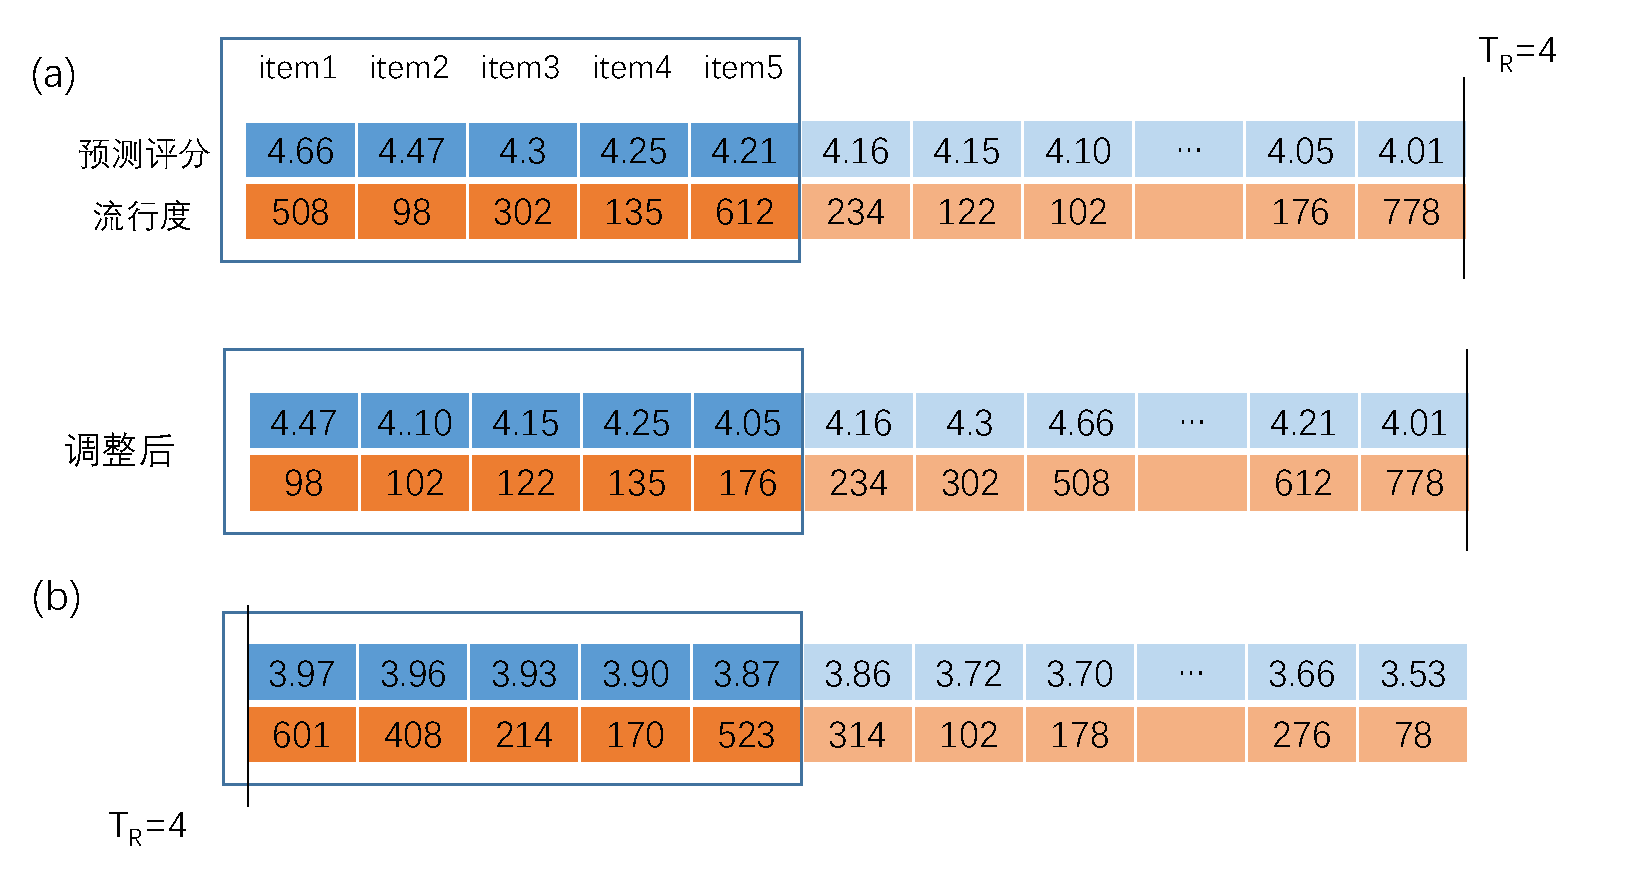
\includegraphics[width=\textwidth]{rerank001_2.eps}\\
  \caption{重排名模型调整示意图}\label{fig:4-3}
\end{figure}
根据改进重排名模型,我们计算出用户$a$的$d_u = 10$,$b_u = 4.1$,用户$b$的$d_u = 40$,$b_u = 3.8$,此时,我们取$\theta = 3$,可以计算出用户$a$的阈值为4.37,用户$b$的$T_R$值为3.89。则按照改进重排名模型调整过后的用户推荐列表如图\ref{fig:4-4}所示,我们可以看到重排名算法对用户$a$和用户$b$的推荐列表都起了作用,且用户$a$兴趣广度较小,推荐列表更多地采用标准排序,准确性更高,而用户$b$兴趣广度较大,推荐列表更多地采用项目流行度排序,多样性更高。这表明,通过考虑用户偏差的改进重排名模型,我们可以针对不同的用户产生不同的阈值,从而可以为用户进行个性化的调整,更好地提升推荐的多样性。
\begin{figure}[htbp]
  \centering
  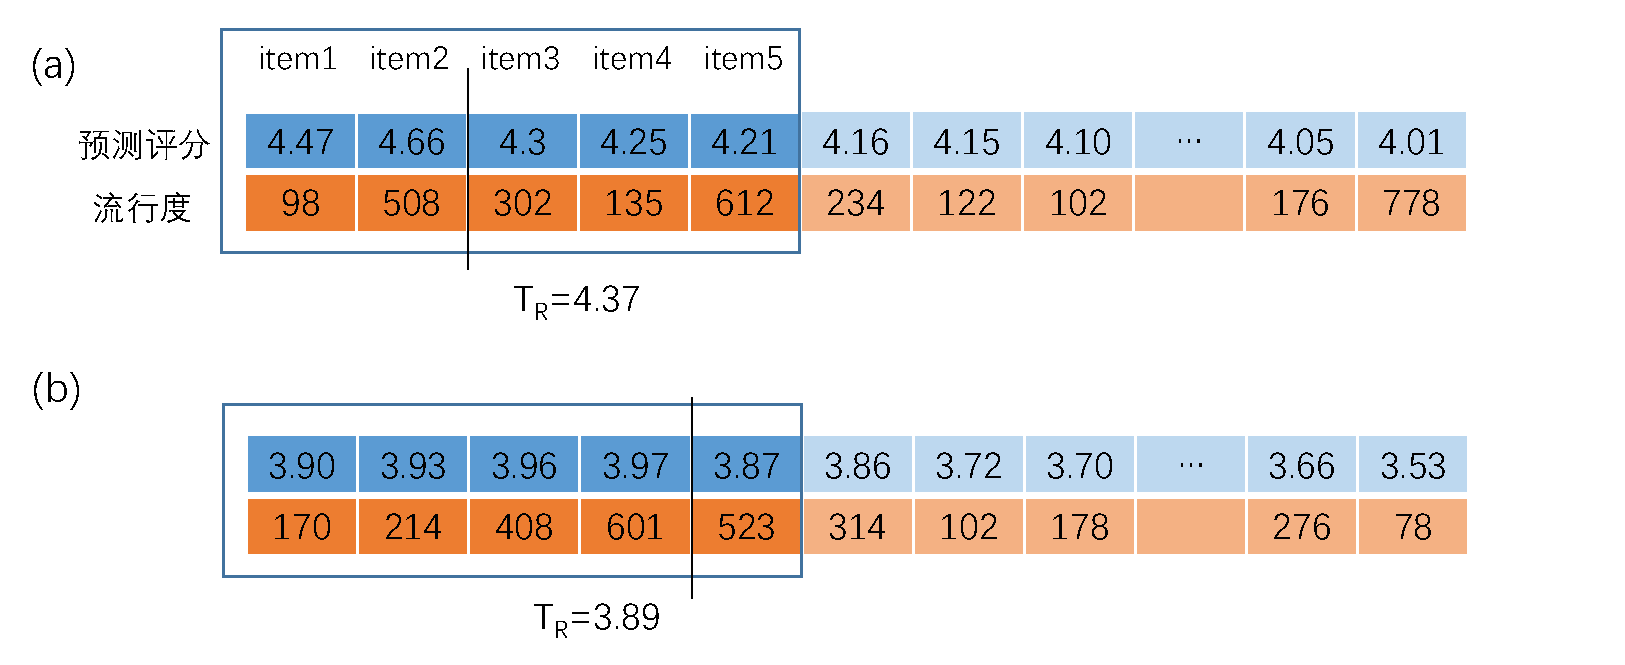
\includegraphics[width=\textwidth]{rerank_final_3.eps}\\
  \caption{改进重排名模型调整示意图}\label{fig:4-4}
\end{figure}

我们的考虑用户偏差的改进重排名算法如下:
\begin{algorithm2e}
	\label{labelpropagation}
	\caption{考虑用户偏差的改进重排名算法}
	\KwIn{ watchlist $W$, average ratings set $M$, $\theta$, $U$, $S$, $m$, $n$}
	\KwOut{recommendation list L}
	\SetKwFunction{GenerateAverageRatingMatrix}{GenerateAverageRatingMatrix}
	\SetKwFunction{GenerateTemporalWeightedMatrix}{GenerateTemporalWeightedMatrix}
	\SetKwFunction{GenerateFrequencyWeightedMatrix}{GenerateFrequencyWeightedMatrix}
	\SetKwFunction{GenerateRatingsMatrix}{GenerateRatingsMatrix}
	\SetKwFunction{GetPredictRatings}{GetPredictRatings}
	\SetKwFunction{SelectTopK}{SelectTopK}

	\textbf{\emph{/*===== Ratings Calculation====*/}}\\
	$A_{m \times n} \gets \GenerateAverageRatingMatrix{$M$}$\;
	$B_{m \times n} \gets \GenerateTemporalWeightedMatrix{$W$}$\;
	$C_{m \times n} \gets \GenerateFrequencyWeightedMatrix{$W$}$\;
	$R_{m \times n} \gets \left( \lambda B_{m \times n}+\left ( 1-\lambda \right )C_{m \times n} \right )\cdot A_{m \times n}$\;

	\textbf{\emph{/*===== Ratings Prediction====*/}}\\
	$P_{m \times n} \gets \GetPredictRatings{$R$}$\;		 
	\textbf{\emph{/*===== Reranking====*/}}

	\For{each $ u \in U $}{
 		compute $b_u$ and  $d_u$\;
 		$T_R(\theta) \gets \min (b_u+\frac{T_{max}-b_u}{d_u}\theta,T_{max})$\;
		\For{ each $s \in S$}{
			\If { $P_{us} \geq T_R(\theta) $}{
				$rank_x(s)$\;
			}
			\Else{
				$rank_{standstard}(s)$\;
			}
		}
		$L \gets \SelectTopK{}$\;
 	}
	
\end{algorithm2e}

我们的改进重排名算法的整体架构如图\ref{fig:4-10}。
\begin{figure}[htbp]
  \centering
  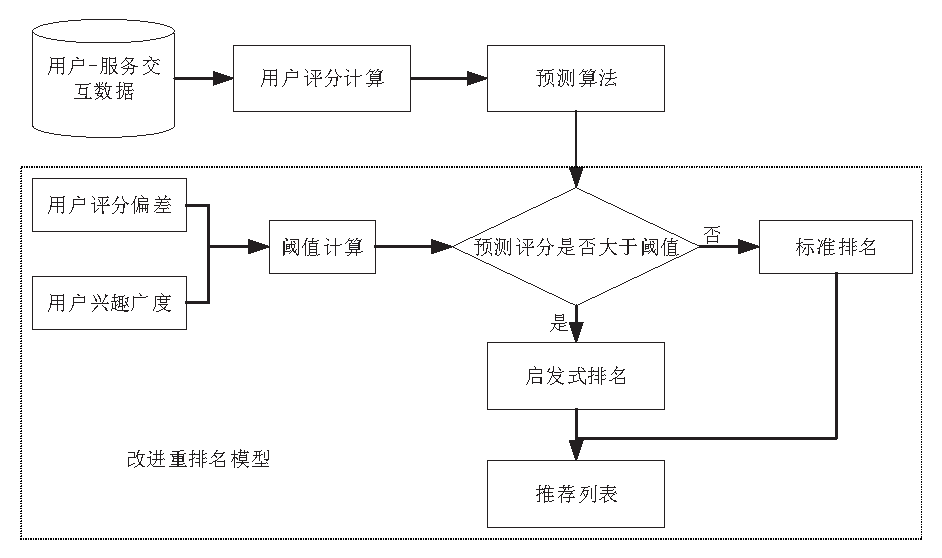
\includegraphics[width=\textwidth]{rerank_kuangjia.eps}\\
  \caption{改进重排名模型框架}\label{fig:4-10}
\end{figure}
\section{算法实现}
我们的改进重排名算法的实现同样基于pweb数据集,我们的算法共分为三个模块,主要是评分计算,评分预测以及重排名三个部分。我们同样是使用Python 2.7作为开发语言来实现了各个模块,由于各模块中有很多部分在第三章已经实现过,所以本章实现的代码量总体不大,约为300行左右。图\ref{fig:4-20}为我们的算法代码模块图,下面将对各模块中主要函数的功能作简要介绍。
\begin{figure}[htbp]
  \centering
  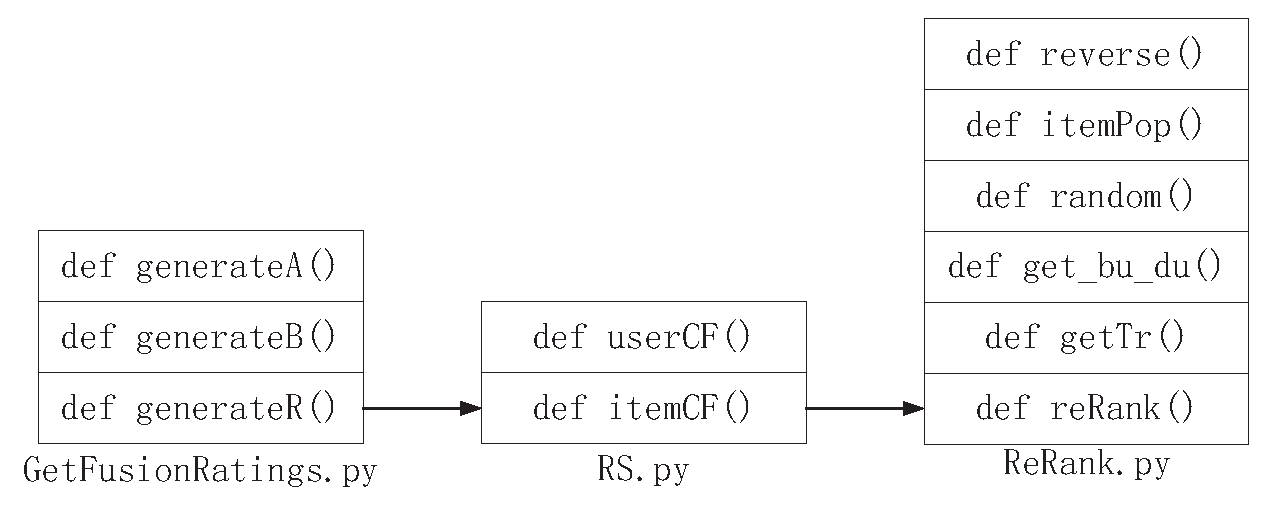
\includegraphics[width=\textwidth]{Code2.eps}\\
  \caption{改进重排名模型代码模块图}\label{fig:4-20}
\end{figure}

\begin{enumerate}
\item \emph{评分计算}~我们在GetFusionRatings.py文件中实现了评分信息的计算,该模块主要有三步,首先我们用第三章的评分计算方法先计算频率权重评分,生成$<user,service,rating_C>$。函数generateA先从数据库中提取所有服务的平均评分,然后给用户观察列表中的服务赋予该服务的平均评分,生成$<user,service,rating_A>$。函数generateB统计用户观察列表中服务首次出现的时间,根据公式\eqref{eq:4-1}生成时间权重评分$<user,service,rating_B>$。函数generateR根据公式\eqref{eq:4-2}产生综合评分$<user,service,rating>$。

\item \emph{评分预测}~我们在RS.py中实现了评分预测模块,分别实现了基于用户的协同过滤userCF函数和基于项目的协同过滤itemCF函数,用以预测用户对服务的评分,这两个函数均使用PCC来计算相似度。

\item \emph{重排名}~函数reverse、itemPop以及random分别是逆序排名、基于项目流行度排名以及随机排名,用以作为启发式的排名方法,函数get\li bu\li du计算用户的平均评分和兴趣广度,函数getTr根据$\theta$来生成阈值$T_R(\theta)$,函数reRank是重排名的过程,首先按照启发式排名进行排序,然后剔除掉评分小于阈值的服务,判断剩下的服务是否达到推荐数,如果达不到,再从剔除的服务中按评分从高到低选取。

\end{enumerate}
\section{实验设计}
\subsection{实验数据及评估指标}
为了验证我们提出的算法在提高Web服务多样性方面的作用,实验依然采用第三章使用的ProgrammableWeb数据集pweb,并且对数据集进行了相同的预处理,即选择watchlist列表中至少包含50个服务或者Mashup的用户,最终我们选择了510个用户和4813个Web服务。

本实验采用精度作为准确性度量的方法,因为本文更多地关注Web服务的总体多样性,因此采用diversity-in-top-N\cite{Ge2010Beyond}作为多样性的评估指标。


\subsection{不同启发式排名方法对比}
重排名方法会对预测评分大于阈值$T_R$的服务使用启发式方法进行重新排序以提高多样性。通常启发式的重排序方法有以下三种:
\begin{enumerate}
\item \emph{逆序排名法(Reverse Rating)}~与标准排名$Rank_{standard}$正好相反,将每个服务的评分从小到大排序,评分越低的服务排名越高。

\item \emph{随机排名法(Random Rating)}~随机选择N个项目进行排名推荐。

\item \emph{项目流行度排名(Item-Popularity Rating)}~将候选项目按照流行度从低到高进行排序,即优先考虑候选服务集中不热门的服务进行推荐。
\end{enumerate}

实验中将数据集的80$\%$用作训练集,20\%用作测试,分别使用基于用户和基于项目的协同过滤来产生预测评分,邻居数设置为50,推荐列表$N$长度设置为5。实验针对上述三种启发式的排名方法,测量了在不同$\theta$取值下,准确性和多样性的变化曲线。
\begin{figure}[htbp]
\centering
\begin{minipage}[t]{0.48\textwidth}
\centering
\includegraphics[width=7cm]{diversity_1.png}
\caption{启发式排名方法在User-Based CF下的准确性和多样性}\label{lab-11}
\end{minipage}
\begin{minipage}[t]{0.48\textwidth}
\centering
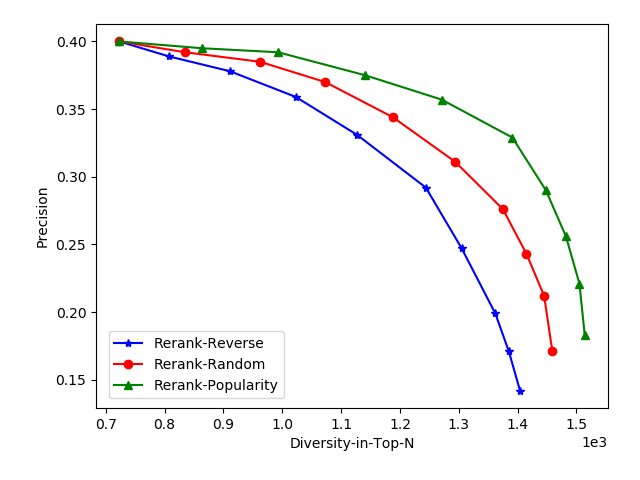
\includegraphics[width=7cm]{diversity_2.png}
\caption{启发式排名方法在Item-Based CF下的准确性和多样性}\label{lab-12}
\end{minipage}
\end{figure}

如图\ref{lab-11},\ref{lab-12}所示,我们可以看到,对于ProgrammableWeb数据集,随着$\theta$的降低,三种启发式排名的方法均可以通过损失一定的准确性来提高多样性,并且初始时损失很小的精度就可以获得较大的多样性性能的提升,随着$\theta$的调节,精度损失越来越大,而多样性性能的提升越来越小。同时,我们发现,在ProgrammableWeb数据集中,以项目流行度作为启发式排名的模型,在损失相同精度的情况下,多样性性能提升最大,这表明通过推荐冷门的服务给用户,能够很好地提升多样性。

进一步地,我们认为仅仅是总体多样性的提高是不够的,我们还希望能够在推荐多样性提高的同时,增加“长尾”服务在推荐中所占的比重,以避免热门的服务越来越们,冷门的服务无人问津的状况。根据“八二定律”,我们将ProgrammableWeb数据集中用户关注数前$20\%$的Web服务称为流行服务,将剩下的服务称为是“长尾”服务。如表\ref{4-1}我们统计了数据集中“长尾”服务和流行服务的数量和用户关注数。我们发现当前ProgrammableWeb网站中用户的关注更多地集中在少量流行服务,关注数前100的服务一共获得了$32.5\%$的分布占比。因此我们在评估多样性提高算法的时候,有必要考察不同算法对“长尾”服务的推荐能力。
\begin{table}[htbp]
\centering
\caption{流行服务和“长尾”服务统计表}\label{4-1}
\begin{tabular}{|c|c|c|}
\hline
服务种类       & 数量   & 用户关注占比 \\ \hline
流行服务       & 962  & 67.9\% \\ \hline
“长尾”服务     & 3851 & 32.1\% \\ \hline
关注数前100的服务 & 100  & 32.5\% \\ \hline
\end{tabular}
\end{table}

我们分别使用基于用户和基于项目的协同过滤来产生预测评分,使用三种启发式排名方法进行重排名,对三种启发式排名方法的“长尾”服务推荐能力进行了验证。实验结果如图\ref{lab-13},\ref{lab-14}所示,横坐标是精度损失,纵坐标是推荐服务总数中“长尾”服务所占的比重。初始状态下推荐结果中“长尾”服务占比只有17$\%$,通过损失很小的精度,三种启发式的排名方法都可以大量提高推荐结果中“长尾”服务的比重,其中项目流行度排名和随机排名提升较大,逆序排名提升较小,这是由于项目流行度排名和随机排名在重排名时,都能更侧重于推荐绝大多数的“长尾”服务。当精度损失达到30$\%$以后,“长尾”服务推荐的比重增长不大,这是由于此时精度损失已经不再能带来多样性的大幅提升。总体而言,基于项目流行度的启发式排名方法可以通过较小的精度损失,让“长尾”服务占比达到50$\%$以上,可以有效地推荐“长尾”服务。

\begin{figure}[htbp]
\centering
\begin{minipage}[t]{0.48\textwidth}
\centering
\includegraphics[width=7cm]{diversity_5.png}
\caption{User-Based CF下的精度损失和“长尾”服务占比}\label{lab-13}
\end{minipage}
\begin{minipage}[t]{0.48\textwidth}
\centering
\includegraphics[width=7cm]{diversity_6.png}
\caption{Item-Based CF下的精度损失和“长尾”服务占比}\label{lab-14}
\end{minipage}
\end{figure}

\subsection{与经典重排名算法的对比}
我们将本文提出的考虑用户偏差的重排名算法与经典的重排名算法进行对比,分别使用基于用户和基于项目的协同过滤来产生预测评分,使用服务流行度排名方法作为启发式排名的方法。实验结果如图\ref{lab-15},\ref{lab-16}所示,我们可以看到,相对于经典的重排名算法,考虑了用户偏差的重排名算法在损失相同的精度的情况下,能够提高更多的总体多样性。在精度损失在12$\%$左右时,我们的方法在总体多样性上相比经典重排名方法提升最大,这可能是由于此时个性化阈值能够恰当的作用在大多数用户身上。而随着精度损失的增大,两种方法在多样性上的提高都在减少,这可能是由于此时阈值对于大多数用户已经失去了调节作用。总体而言,考虑用户偏差的重排名方法能够在较少损失精度的情况下,较大地提升多样性。
\begin{figure}[htbp]
\centering
\begin{minipage}[t]{0.48\textwidth}
\centering
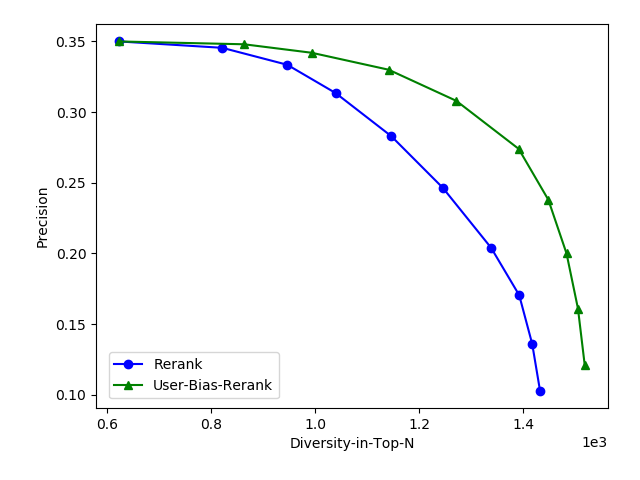
\includegraphics[width=7cm]{diversity_3.png}
\caption{User-Based CF下两种算法准确性和多样性对比}\label{lab-15}
\end{minipage}
\begin{minipage}[t]{0.48\textwidth}
\centering
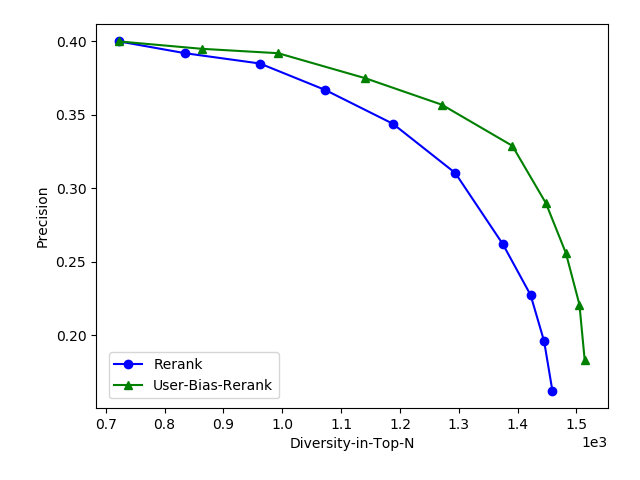
\includegraphics[width=7cm]{diversity_4.png}
\caption{Item-Based CF下两种算法准确性和多样性对比}\label{lab-16}
\end{minipage}
\end{figure}

\begin{figure}[htbp]
\centering
\begin{minipage}[t]{0.48\textwidth}
\centering
\includegraphics[width=7cm]{diversity_7.png}
\caption{User-Based CF下两种算法精度损失和“长尾”服务占比}\label{lab-17}
\end{minipage}
\begin{minipage}[t]{0.48\textwidth}
\centering
\includegraphics[width=7cm]{diversity_8.png}
\caption{Item-Based CF下两种算法精度损失和“长尾”服务占比}\label{lab-18}
\end{minipage}
\end{figure}

同样地,我们考察了两种算法对“长尾”服务的推荐能力,实验结果如图\ref{lab-17},\ref{lab-18}所示,初始时两种算法都可以在损失少量精度的情况下,大幅提升推荐列表中“长尾”服务的比重,且我们的算法在提升比例上要高于经典的重排名算法。当精度损失超过30$\%$时,“长尾”服务提升占比不再能大幅提升,且两种算法提升比例趋于接近,这是由于此时阈值对不同用户的调节作用在减弱,两种算法的差异性在减小。总体而言,相对于经典重排名算法,我们的算法在损失精度较小的时候,可以较大地提高“长尾”服务的比例。通过少量损失精度,可以将“长尾”服务的占比增加到50$\%$左右。



\section{本章小结}
本章我们阐述了服务推荐中引入推荐多样性的意义,并提出了一种考虑用户偏差的改进重排名算法,该算法在重排名算法的基础上,考虑了不同用户在评分习惯和兴趣分布上的差异性,从而更好地在准确性和多样性之间取得平衡。基于ProgrammableWeb网站的用户数据实验表明,本章的方法可以在较少地损失推荐准确性的同时,较大地提升推荐多样性,为用户推荐更加多样化的Web服务。

%%%%%%%%%%%%%%%%%%%%%%%%%%%%%%%%%%%%%%%%%%%%%%%%%%%%%%%%%%%%%%%%%%%%%%%%%%%%%%%

%%%%%%%%%%%%%%%%%%%%%%%%%%%%%%%%%%%%%%%%%%%%%%%%%%%%%%%%%%%%%%%%%%%%%%%%%%%%%%%
% 学位论文的正文应以《结论》作为最后一章
\chapter{总结与展望}\label{5}
\section{工作总结}
随着面向服务架构的发展,互联网上涌现了大量的Web服务,如何为用户推荐合适的服务成为了当务之急。当前的服务推荐工作大都基于服务质量QoS或者用户的历史偏好信息,Web服务丰富的边缘信息没有得到很好地利用。同时,当前的Web服务的相关研究工作,往往只关注了服务推荐的准确性,而忽略了推荐的多样性。本文鉴于当前研究的不足,基于服务平台ProgrammaleWeb的用户真实的历史偏好信息来发掘用户兴趣,在服务推荐的准确性和多样性方面作了如下工作:

\begin{enumerate}
\item 在服务推荐的准确性方面,提出了一种融合主题信息和服务组合信息的Web服务推荐算法,该算法基于ProgrammableWeb网站的真实数据,通过用户的隐式反馈信息来提取用户的兴趣偏好,通过ProgrammableWeb网站的服务注册页面来提取服务的功能描述信息以及服务组合信息,并以此分别计算了Web服务之间在主题以及服务组合关系上的相似度,并根据相似度获取了每个Web服务在主题或者服务组合上的邻居Web服务集合,将其与SVD矩阵分解模型相结合,以预测用户评分的缺失值。实验表明,相对于SVD模型和引入时间信息的SVD模型,我们的算法在准确性上取得了一定的提升,这表明引入主题信息和服务组合信息的对提升推荐的准确性是有效的。

\item 在服务推荐的多样性方面,提出了一种考虑用户偏差的改进重排名算法以提高推荐的多样性。该算法在经典的重排名算法的基础上,考虑了用户的评分习惯的差异性和兴趣分布差异性,并将这两种偏差结合进了阈值$T_R$的计算中,使得改进的重排名模型不再按照固定阈值$T_R$,而是通过考虑了用户差异性的个性化阈值来为用户提高多样性。该算法不依赖于具体的推荐算法,可以方便地与其他推荐模型相结合。实验表明,考虑用户偏差的改进重排名算法,可以在尽量少降低准确性的情况下,大幅提升推荐的多样性。
\end{enumerate}

\section{研究展望}
本文基于ProgrammableWeb网站的用户真实历史偏好信息,在服务推荐的准确性和多样性方面进行了研究,但是由于时间和精力有限,本文的工作还有很多可以提高的地方:

\begin{enumerate}
\item 在准确性方面,本文主要考虑了主题信息和服务组合信息,而对于用户间的关系,例如用户的社交关系没有进行考虑。同时,时间信息也是推荐中一个比较重要的因素。未来考虑在模型中综合考虑用户间的社交关系以及时间信息,使得推荐更加多元化。

\item 在多样性方面,本文在经典的重排名算法的基础上,考虑了用户的差异性,可以尽量少地降低精度的情况下,尽量多地提高推荐的多样性,但是这种方法不是一种最大化多样性的方法。因此未来考虑在允许一定精度损失的情况下,以最大化Web服务推荐的多样性为优化目标进行研究。

\item 本文主要致力于服务推荐算法的研究,未来考虑将本文的算法集成到一个推荐系统中,增加系统的交互性,更好地进行推荐。

\end{enumerate}



%%%%%%%%%%%%%%%%%%%%%%%%%%%%%%%%%%%%%%%%%%%%%%%%%%%%%%%%%%%%%%%%%%%%%%%%%%%%%%%
% 致谢,应放在《结论》之后
\begin{acknowledgement}
时间如白驹过隙,转眼间三年时间已经过去,研究生的学习生活也即将结束。在这三年的时间里,我的学习和生活都离不开老师和同学们的各种帮助,在此我要向他们致以最诚挚的谢意。

感谢我的导师胡昊副教授。无论是学习上还是生活上,胡昊老师都给我提供了非常多的帮助。本文从选题、实验到成文都离不开胡老师的悉心指导。胡老师幽默风趣的谈吐和一丝不苟的科研态度,都给我留下了深刻的印象,让我受益匪浅。

感谢南京大学软件研究所的各位老师。感谢吕建教授、马晓星教授、陶先平教授、徐锋教授、许畅教授、黄宇教授、曹春副教授、余萍副教授、马骏老师、张建莹老师、徐经纬老师、汪亮老师、姚远老师、蒋炎岩老师、魏恒峰老师、匡宏宇老师等所有关心和帮助过我的老师。感谢你们在这研究生三年对我的指导和关怀,你们的言传身教将会是我一生最宝贵的财富。

感谢软件所所有的同学们,特别是张宗飞、孟占帅同学,非常荣幸能够和这些优秀的同学一起奋斗,一起度过人生最难忘的三年。感谢我的舍友吴少博同学在我的生活上的关心和帮助,让我即使远离家乡也能感受到家庭般的温馨。

最后我要感谢我的家人,你们一直是我最坚强的后盾,我的一路成长离不开你们的支持和鼓励。你们是我心灵的港湾,是我不断前进的动力。
\end{acknowledgement}

%%%%%%%%%%%%%%%%%%%%%%%%%%%%%%%%%%%%%%%%%%%%%%%%%%%%%%%%%%%%%%%%%%%%%%%%%%%%%%%
% 附录
\appendix





% 参考文献。应放在\backmatter之前。
% 推荐使用BibTeX,若不使用BibTeX时注释掉下面一句。
\nocite{*}
\bibliography{sample}
% 不使用 BibTeX
%\begin{thebibliography}{2}
%
%\bibitem{deng:01a}
%{邓建松,彭冉冉,陈长松}.
%\newblock {\em \LaTeXe{}科技排版指南}.
%\newblock 科学出版社,书号:7-03-009239-2/TP.1516, 北京, 2001.
%
%\bibitem{wang:00a}
%王磊.
%\newblock {\em \LaTeXe{}插图指南}.
%\newblock 2000.
%\end{thebibliography}

% 附录,必须放在参考文献后,backmatter前
\appendix

%%%%%%%%%%%%%%%%%%%%%%%%%%%%%%%%%%%%%%%%%%%%%%%%%%%%%%%%%%%%%%%%%%%%%%%%%%%%%%%
% 书籍附件
\backmatter
%%%%%%%%%%%%%%%%%%%%%%%%%%%%%%%%%%%%%%%%%%%%%%%%%%%%%%%%%%%%%%%%%%%%%%%%%%%%%%%
% 作者简历与科研成果页,应放在backmatter之后
\begin{resume}
% 论文作者身份简介,一句话即可。
\begin{authorinfo}
\noindent 王勇,男,汉族,1993年4月出生,江苏省泰州人。
\end{authorinfo}
% 论文作者教育经历列表,按日期从近到远排列,不包括将要申请的学位。
\begin{education}
\item[2015年9月 --- 2018年9月] 南京大学计算机科学与技术系 \hfill 硕士
\item[2011年9月 --- 2015年6月] 南京大学计算机科学与技术系 \hfill 本科
\end{education}
% 论文作者在攻读学位期间所发表的文章的列表,按发表日期从近到远排列。
\begin{publications}
\item 胡昊,王勇。 专利“一种基于主题和服务组合信息的Web服务推荐方法”。申请号:201810424947.3。
\end{publications}
% 论文作者在攻读学位期间参与的科研课题的列表,按照日期从近到远排列。
\end{resume}

%%%%%%%%%%%%%%%%%%%%%%%%%%%%%%%%%%%%%%%%%%%%%%%%%%%%%%%%%%%%%%%%%%%%%%%%%%%%%%%
% 生成《学位论文出版授权书》页面,应放在最后一页
\makelicense

%%%%%%%%%%%%%%%%%%%%%%%%%%%%%%%%%%%%%%%%%%%%%%%%%%%%%%%%%%%%%%%%%%%%%%%%%%%%%%%
\end{document}
